\appendix
\chapter{Appendix for COINs}

\section{Theory}
\label{sec:appendix_proofs}

\begin{proof}[Proposition~\ref{proposition:complexity}]
    The time complexity of the first node group prediction step of the new evaluation procedure, is proportional to the number of groups $K$, as this is the number of embeddings required. On the other hand, the second step requires as many model evaluations as the number of nodes in the group, $\abs{C_k}$. For each sample, the total is thus $K+\abs{C_k}$, while each node group is represented by $N_k^{\text{test}}$ samples in the test data. By summing over all groups $k$ one obtains the provided exact complexity.

    Regarding the expression $\sum_{k=1}^{K}{\of{K+\abs{C_k}}N_k^{\text{test}}}$, let us first assume that we have fixed the number of groups $K$ to some value in $\offf{1,\dots,\abs{V}}$ and we are aiming to optimize the distribution of nodes and evaluation samples across groups for this fixed $K$. Using the KKT theorem, one can prove that extremal configurations only occur when all groups are of equal size and/or all groups are represented with an equal amount of samples in the evaluation set. Lemma~\ref{lemma:kkt_evaluation_cost} gives the details. It is easier to strive towards $\abs{C_k} \approx \frac{\abs{V}}{K}$, however, in any case, the number of node embedding computations will then equal $N\of{K + \frac{\abs{V}}{K}}$. 
    
    To conclude, we prove that the value of $K$ is what decides whether the lower or upper bound stated above is achieved: $K=\sqrt{V}$ gives the motivating lower bound, while $K \in \offf{1, \abs{V}}$ produces the worst performance, which is in the same order as the baseline $N \abs{V}$. Lemma~\ref{lemma:min_max_evaluation_cost} gives the details.
\end{proof}

\begin{lemma}
    \label{lemma:kkt_evaluation_cost}
    Let $\offf{a_k}_{k=1}^{K}=\offf{\abs{C_k}}_{k=1}^{K}$ and $\offf{b_k}_{k=1}^{K}=\offf{N_k^{\text{test}}}_{k=1}^{K}$ denote the learnable parameters. Then with the constraints $$\sum_{k=1}^{K}{a_k}=\abs{V}, \sum_{k=1}^{K}{b_k}=N, \forall k, a_k > 0, b_k \geq 0,$$ the only extremal points of $g\of{\offf{a_k},\offf{b_k}}=\sum_{k=1}^{K}{\of{K + a_k}b_k}$ are $\forall k, a^*_k = \frac{\abs{V}}{K}$ and/or $\forall k, b^*_k = \frac{N}{K}$, with the extreme value of $g\of{\offf{a^*_k},\offf{b^*_k}}=N\of{K + \frac{\abs{V}}{K}}$.
\end{lemma}
    \begin{proof}
        The Lagrangian of the optimization problem is the following:
        \begin{align*}
             L\of{\offf{a_k},\offf{b_k}} &= \sum_{k=1}^{K}{\of{K + a_k}b_k} + \lambda_1 \of{\sum_{k=1}^{K}{a_k} - \abs{V}} + \lambda_2 \of{\sum_{k=1}^{K}{b_k} - N} \\
             &- \sum_{k=1}^{K}{\mu_k a_k} - \sum_{k=1}^{K}{\nu_k b_k}
        \end{align*}
        $$$$
    From the stationarity KKT conditions:
    \begin{align*}
        \forall k, \frac{\partial L}{\partial a_k} &= 0 \Leftrightarrow \forall k, b_k + \lambda_1 - \mu_k = 0 \Leftrightarrow  \forall k, b_k = \mu_k - \lambda_1 \\
        \forall k, \frac{\partial L}{\partial b_k} &= 0 \Leftrightarrow \forall k, a_k + K + \lambda_2 - \nu_k = 0, \Leftrightarrow \forall k, a_k = \nu_k - \lambda_2 - K
    \end{align*}
    Now, by the primal equality constraints:
    \begin{align*}
        \sum_{k=1}^{K}{a_k} &= \abs{V} \Leftrightarrow \sum_{k=1}^{K}{\of{\nu_k - \lambda_2 - K}} = \abs{V} \Leftrightarrow \lambda_2 = \frac{1}{K} \sum_{k=1}^{K}{\nu_k} - \frac{\abs{V}}{K} - K \\
        \Rightarrow \forall k, a_k &= \nu_k - \frac{1}{K} \sum_{j=1}^{K}{\nu_j} + \frac{\abs{V}}{K} \\
        \sum_{k=1}^{K}{b_k} &= N \Leftrightarrow \sum_{k=1}^{K}{\of{\mu_k - \lambda_1}} = N \Leftrightarrow \lambda_1 = \frac{1}{K} \sum_{k=1}^{K}{\mu_k} - \frac{N}{K} \\
        \Rightarrow \forall k, b_k &= \mu_k - \frac{1}{K} \sum_{j=1}^{K}{\mu_j} + \frac{N}{K}
    \end{align*}
    Finally, by the complementary slackness KKT conditions, primal inequality constraints, and dual feasibility KKT conditions:
    \begin{align*}
        \sum_{k=1}^{K}{\mu_k a_k} &= 0 \Leftrightarrow \forall k, \mu_k = 0 \Rightarrow \forall k, b^*_k=\frac{N}{K} & \text{ as $\forall k, a_k>0,\mu_k \geq 0$}\\
        \sum_{k=1}^{K}{\nu_k b_k} &= 0 \Leftarrow \forall k, \nu_k = 0 \Rightarrow \forall k, a^*_k = \frac{\abs{V}}{K} & \text{ as $\forall k, b_k \geq 0,\nu_k \geq 0$}
    \end{align*}
    \end{proof}

\begin{lemma}
    \label{lemma:min_max_evaluation_cost}
    By choosing $K=\sqrt{\abs{V}}$, one achieves the minimal evaluation cost $2 N \sqrt{\abs{V}}$, while with $K \in \offf{1, \abs{V}}$ one achieves the maximum $N\of{\abs{V} + 1}$.
\end{lemma}
\begin{proof}
    Let $f\of{K} = N\of{K + \frac{\abs{V}}{K}}$. Then note that $f'\of{K} = N - \frac{N \abs{V}}{K^2}$. From this, we find the only critical point of $f$ in $\of{1, \abs{V}}$: 
    
    $N - \frac{N \abs{V}}{K^2} = 0 \Leftrightarrow K^2 = \frac{N \abs{V}}{N} \Leftrightarrow K = \sqrt{\abs{V}}$. 
    
    Now $f''\of{K}=\frac{2 N \abs{V}}{K^3}$. As $\forall K \in \off{1, \abs{V}}, f''\of{K} > 0$, $f$ is a convex function for all values of $K$. Thus, $\sqrt{\abs{V}}$ will be both a local and global minimum, while the endpoints of the interval will be global maxima, as $\forall K \neq \sqrt{\abs{V}}, f'\of{K} > 0$, i.e., $f$ increases away from the minimum in both directions.
\end{proof}


\begin{proposition}
    \label{proposition:condition_applicability}
    Let $C \in \offf{1,\dots,K}$ be a r.v. storing from which community a sample belongs. Let $\forall k \in \offf{1,\dots,K}, H'_k \in \offf{1,\dots\,\abs{C_k}}$ be the r.v. counting how many samples need to be evaluated before a correct hit in community $k$ is achieved by COINs, with $\forall k, H_k$ counting the same for the baseline model. 
    
    Let $\forall k, T'_k=K+\abs{C_k}$ denote the number of embedding computations required for evaluating a sample in community $k$ (recall Proposition~\ref{proposition:complexity}), with $T_k=\abs{V}$ counting the same for the baseline model. 
    
    Let $\forall k, \bar{\rho}'_k$ be the evaluated mean rank for samples from community $k$ for COINs, with $\bar{\rho}$ denoting the baseline mean rank. 
    
    Finally, let $\forall k, \varepsilon_k = \frac{\bar{\rho}'_k - \bar{\rho}}{\bar{\rho}}$ denote the per-community relative error in mean rank incurred to the baseline after training and evaluating the model with COINs, while let $\forall k, A_k=\frac{T_k}{T'_k}=\frac{\abs{V}}{K+\abs{C_k}}$ denote the per-community acceleration achieved. 
    
    Then, if we assume that:
    \begin{itemize}
        \item $\forall k, \mathbb{P}\of{C=k}=\frac{N_k^{\text{test}}}{N}$, and
        \item $\forall j \in \offf{1,\dots\,\abs{C_k}}, \mathbb{P}\of{H_k \leq j}=\of{\text{Hits@j}}_k$,
    \end{itemize}
     the application of COINs is justified if:
    \begin{equation}
        \label{eq:condition_applicability}
        \sum_{k=1}^{K}{\frac{N_k^{\text{test}}}{N} \frac{1 + \varepsilon_k}{A_k}} < 1
    \end{equation}
\end{proposition}
\begin{proof}
The better model is deemed the one with lower overall expected cost up until a correct hit:
    \begin{align*}
        \mathbb{E}\off{T' H'} &< \mathbb{E}\off{T H} \\
        \Leftrightarrow \sum_{k=1}^{K}{\frac{N_k^{\text{test}}}{N} T'_k \bar{\rho}'_k} &< T \bar{\rho}, & \text{ by Lemma~\ref{lemma:expected_evaluations}} \\
        \Leftrightarrow \sum_{k=1}^{K}{\frac{N_k^{\text{test}}}{N} \frac{1 + \varepsilon_k}{A_k}} &< 1, & \text{ after dividing by RHS}
    \end{align*}
\end{proof}%

\begin{lemma}
    \label{lemma:expected_evaluations}
    Let $C \in \offf{1,\dots,K}$ be a r.v. storing from which community a sample belongs. Let $H$ be the r.v. counting how many queries were evaluated before a correct hit is achieved and let $F$ denote the r.v. counting the number of embedding computations required for evaluating a sample. Then:
    $$\mathbb{E}\off{T H} = \sum_{k=1}^{K}{\frac{N_k^{\text{test}}}{N} T_k \bar{\rho}_k}$$
\end{lemma}
\begin{proof}
    \begin{align*}
        &\mathbb{E}\off{T H} = \mathbb{E}_{C}\off{\mathbb{E}\off{T H \mid C}}%, & \text{ by the Law of Total Expectation} 
        %\\
        %&
        = \sum_{k=1}^{K}{\mathbb{E}\off{T H \mid C=k} \mathbb{P}\of{C=k}}%, & \text{ by definition and the LOTUS} 
        \\
        &= \sum_{k=1}^{K}{T_k \mathbb{E}\off{H_k} \mathbb{P}\of{C=k}}%, & \text{ by definition and linearity of exp.} 
        %\\
        %&
        = \sum_{k=1}^{K}{\mathbb{P}\of{C=k} T_k \sum_{j=1}^{\abs{C_k}}{j \mathbb{P}\of{H_k=j}}}%, & \text{ by definition} 
        \\
        &= \sum_{k=1}^{K}{\mathbb{P}\of{C=k} T_k \sum_{j=1}^{\abs{C_k}}{j \off{\mathbb{P}\of{H_k \leq j} - \mathbb{P}\of{H_k \leq j-1}}}}%, & \text{ since $H_k$'s are discrete r.v.s} 
        \\
        &= \sum_{k=1}^{K}{\mathbb{P}\of{C=k} T_k \off{\abs{C_k}- \sum_{j=1}^{\abs{C_k}-1}{\mathbb{P}\of{H_k \leq j}}}}%, & \text{ after cancelling out the telescoping} 
        \\
        &= \sum_{k=1}^{K}{\frac{N_k^{\text{test}}}{N} T_k \off{\abs{C_k}- \sum_{j=1}^{\abs{C_k}-1}{\of{\text{Hits@j}}_k}}}%, & \text{ by the assumptions} 
        \\
        &= \sum_{k=1}^{K}{\frac{N_k^{\text{test}}}{N} T_k \off{\abs{C_k}- \sum_{j=1}^{\abs{C_k}-1}{\frac{1}{N_k^{\text{test}}}\sum_{i \mid c\of{a_i}=k}{\mathbb{I}\of{\rho^{\of{i}} \leq j}}}}}%, & \text{ by definition} 
        \\
        &= \sum_{k=1}^{K}{\frac{N_k^{\text{test}}}{N} T_k \off{\abs{C_k}- \frac{1}{N_k^{\text{test}}}\sum_{i \mid c\of{a_i}=k}{\of{\abs{C_k}- \rho^{\of{i}}}}}}%, & \text{ after switching sum order} 
        \\
        &= \sum_{k=1}^{K}{\frac{N_k^{\text{test}}}{N} T_k \off{\abs{C_k}- \abs{C_k} + \frac{1}{N_k^{\text{test}}}\sum_{i \mid c\of{a_i}=k}{\rho^{\of{i}}}}}%, & \text{ after distributing} 
        \\
        % &= \sum_{k=1}^{K}{\frac{N_k^{\text{test}}}{N} T_k \off{\abs{C_k}- \abs{C_k} + \bar{\rho}_k }}, & \text{ by definition} \\
        &= \sum_{k=1}^{K}{\frac{N_k^{\text{test}}}{N} T_k \bar{\rho}_k}%, & \text{ by definition}
    \end{align*}
    If $\forall k, T_k = T$ like for the baseline models, then:
    \begin{align*}
        \mathbb{E}\off{T H} &= T \sum_{k=1}^{K}{\frac{N_k^{\text{test}}}{N} \bar{\rho}_k}%, & \text{ by linearity of expectation and everything before} 
        %\\ 
        %&
        = T \sum_{k=1}^{K}{\frac{N_k^{\text{test}}}{N} \frac{1}{N_k^{\text{test}}}\sum_{i \mid c\of{a_i}=k}{\rho^{\of{i}}}}%, & \text{ by definition} 
        \\
        &= T \frac{1}{N} \sum_{i=1}^{N}{\rho^{\of{i}}}%, & \text{ after cancelling and combining the sums} 
        %\\
        %&
        = T \bar{\rho}%, & \text{ by definition}
    \end{align*}
\end{proof}

\begin{proof}[Proposition \ref{proposition:complexity_distributed}]
    To explain the complexity, we note that in a parallel computing setting, where we assume equal computation power for each machine, the overall cost of Step 2 is equal to that of the machine who will do the most work (in this case the most node-level query-answer embeddings computed). The additional $KN$ term is the total cost of Step 1, which is not parallelized.

    The largest overall cost is naturally achieved when $\abs{U}=1$, i.e. we fall back to the single-machine setting without parallelization, thus the upper bound is the same as before.

    The lower bound requires a new argument based on calculus. To start, the obvious lower bound to the maximum cost across machines is the minimum cost. We would achieve this lower bound when the max and min are equal, i.e. only when each machine does the same amount of work. In our case, this quantity is $\textcolor{blue}{\frac{1}{\abs{U}}}\sum_{k=1}^{K}{\abs{C_k}N_k^{\text{test}}}$. If we keep $\abs{U}$ and $K$ fixed as constants, we can use the KKT result from the proof of Proposition \ref{proposition:complexity} and deduce that now the only extremal points will have the form $N\of{K+\frac{\abs{V}}{K\textcolor{blue}{\abs{U}}}}$. Note that we have the constraints $1 \leq K \leq \abs{V}$ and $1 \leq \abs{U} \leq K$ (having more machines than communities is useless).

    Let $f\of{K, \abs{U}}=N\of{K+\frac{\abs{V}}{K\abs{U}}}$. Then $\nabla f \of{K, \abs{U}}=\of{\frac{\partial f}{\partial K},\frac{\partial f}{\partial \abs{U}}}=\of{N\of{1-\frac{\abs{V}}{K^2\abs{U}}}, -N\frac{\abs{V}}{K\abs{U}^2}})$.

    Setting $\nabla f = \of{0, 0}$ yields that we must have $K^2\abs{U}=\abs{V}$ and $K\abs{U}^2 \to \infty$, which is impossible with the constraints. So the only critical points can be boundary points:
    \begin{itemize}
        \item The corners $\offf{\of{1, 1}, \of{\abs{V}, 1}, \of{\abs{V},\abs{V}}}$;
        \item On the line $\abs{U}=1$, we know $K=\sqrt{\abs{V}}$ is a local minimum;
        \item On the line $K=\abs{V}$, $f\of{K, \abs{U}}=N\of{\abs{V}+\frac{1}{\abs{U}}}$ simply monotonically decreases with $\abs{U}$, so there is no local minimum on this line;
        \item On the line $\abs{U}=K$, $f\of{K, \abs{U}}=N\of{K+\frac{\abs{V}}{K^2}}$. So $\frac{d f}{d K}=N\of{1-\frac{2\abs{V}}{K^3}}$. Setting $\frac{d f}{d K}=0$ yields the local minimum $K=\sqrt[3]{2\abs{V}}$ on this line.
    \end{itemize}
    So the full set of global minimum candidates is: $$\of{K^*, \abs{U}^*} \in \offf{\of{1, 1}, \of{\abs{V}, 1}, \of{\abs{V},\abs{V}}, \of{\sqrt{\abs{V}}, 1}, \of{\sqrt[3]{2\abs{V}}, \sqrt[3]{2\abs{V}}} }.$$ Out of all of them, using both $\sqrt[3]{2\abs{V}}$ communities and machines yields the minimal function value of $\frac{3}{2}N\sqrt[3]{2\abs{V}}$.
\end{proof}

\section{Balanced Partitioning for Distributed COINs}
\label{sec:appendix_balanced_partition_algs}

Algorithm \ref{algorithm:balanced_partition} details the optimal solution to the balanced partition problem using top-down dynamic programming, while Algorithm \ref{algorithm:balanced_partition_greedy} displays the scalable greedy method.

\begin{algorithm}[H]
\algsetup{linenosize=\tiny}
\scriptsize
\caption{Exact Balanced Partition}
\label{algorithm:balanced_partition}
\begin{algorithmic}[1]
\STATE{\textbf{input} $\offf{p_k}_{k=1}^{K+1}$, $U=\offf{u_1,u_2,\dots}$}
\STATE{$S \gets \sum_{k=1}^{K+1}{p_k}$}
\STATE{MEMO$\gets\offf{}$}
\STATE{\textbf{function} $\text{MinCost}\of{k,\offf{s_j}_{j=1}^{\abs{U}-1}}$:}
% \bindent
\IF{$\of{k,\offf{s_j}_{j=1}^{\abs{U}-1}}\notin$ MEMO}
% \bindent
\IF{$k=K+2$}
% \bindent
\STATE{$\mu\gets\max\of{\max_{j=1}^{\abs{U}-1}{s_j},S-\sum_{j=1}^{\abs{U}-1}{s_j}}$}
% \eindent
\ELSE
% \bindent
\STATE{$\mu\gets\text{MinCost}\of{k+1,\offf{s_j}_{j=1}^{\abs{U}-1}}$}
\FOR{$i \leftarrow 1$ to $\abs{U}-1$}
% \bindent
\STATE{$\mu\gets\min\of{\mu, \text{MinCost}\of{k+1,\offf{s_j}_{j=1}^{i-1}\cup\offf{s_i+p_k}\cup\offf{s_j}_{j=i+1}^{\abs{U}-1}}}$}
% \eindent
\ENDFOR
% \eindent
\ENDIF
% \eindent
\STATE{MEMO$\off{\of{k,\offf{s_j}_{j=1}^{\abs{U}-1}}}\gets\mu$}
\ENDIF
\RETURN{MEMO$\off{\of{k,\offf{s_j}_{j=1}^{\abs{U}-1}}}$}
% \eindent
\STATE{\textbf{end} MinCost}
\STATE{$\mu^*\gets$MinCost$\of{1, \offf{0}_{j=1}^{\abs{U}-1}}$}
\STATE{$\offf{s^*_j}_{j=1}^{\abs{U}-1}\gets\offf{0}_{j=1}^{\abs{U}-1}$}
\FOR{$k \leftarrow 1$ to $K+1$}
\STATE{$i^*\gets\abs{U}$}
\FOR{$i \leftarrow 1$ to $\abs{U}-1$}
\IF{MEMO$\off{\of{k+1, \offf{s^*_j}_{j=1}^{i-1}\cup\offf{s^*_j+p_k}\cup\offf{s^*_j}_{j=i+1}^{\abs{U}-1}}}=\mu^*$}
\STATE{$i^*\gets i$}
\ENDIF
\ENDFOR
\STATE{$s_{i^*}^*\gets s_{i^*}^*+p_k$}
\IF{$k=K+1$}
\STATE{$u\of{g_V^*}\gets u_{i^*}$}
\ELSE
\STATE{$u\of{g_V^k}\gets u_{i^*}$}
\ENDIF
\ENDFOR
\end{algorithmic}
\end{algorithm}

\begin{algorithm}[H]
% \algsetup{linenosize=\tiny}
% \scriptsize
\caption{Greedy Balanced Partition}
\label{algorithm:balanced_partition_greedy}
\begin{algorithmic}[1]
\STATE{\textbf{input} $\offf{p_k}_{k=1}^{K+1}$, $U=\offf{u_1,u_2,\dots}$}
\STATE{$h_C\gets\text{MaxHeap}\of{\offf{\of{p_k,k}}_{k=1}^{K+1}}$}
\STATE{$h_U\gets\text{MinHeap}\of{\offf{\of{0,j}}_{j=1}^{\abs{U}}}$}
\FOR{$l \leftarrow 1$ to $K+1$}
\STATE{$\of{p_k^*,k^*}\gets\text{HeapPop}\of{h_C}$}
\STATE{$\of{s_i^*,i^*}\gets\text{HeapPop}\of{h_U}$}
\IF{$k^*=K+1$}
\STATE{$u\of{g_V^*}\gets u_{i^*}$}
\ELSE
\STATE{$u\of{g_V^{k^*}}\gets u_{i^*}$}
\ENDIF
\STATE{$\text{HeapPush}\of{h_U,\of{s_i^*+p_k^*,i^*}}$}
\ENDFOR
\end{algorithmic}
\end{algorithm}


\section{Hyperparameters}
\label{sec:appendix_hpars}

Table~\ref{tab:hyperparameters} lists the chosen values of the main hyperparameters influencing community detection, model architecture and optimization.

\begin{table}[ht!]
  \caption[COINs hyperparameter configurations.]{COINs hyperparameter configurations. Left to right: Leiden resolution, embedding dimension, contrastive loss margin, COINs loss weight, mini-batch size, number of negative samples per positive, total number of training epochs, learning rate, and regularization weight.}
  \label{tab:hyperparameters}
  \centering
  \begin{tabular}{llccccccccc}
    \toprule
    Dataset & Model & resolution & $D$ & $\gamma$ & $\alpha$ & $B$ & $m$ & ep. & l.r. & $\lambda$ \\
    \midrule
\multirow{6}{*}{FB15k-237} & TransE & $5 \cdot 10^{-3}$ & 100 & 1.0 & 0.5 & 256 & 128 & 5 & $10^{-3}$ & $10^{-6}$ \\
 & DistMult & $5 \cdot 10^{-3}$ & 100 & \textemdash & 0.5 & 256 & 128 & 50 & $10^{-3}$ & $10^{-6}$ \\
 & ComplEx & $5 \cdot 10^{-3}$ & 100 & \textemdash & 0.5 & 256 & 128 & 50 & $10^{-3}$ & $10^{-6}$ \\
 & RotatE & $5 \cdot 10^{-3}$ & 100 & 9.0 & 0.5 & 256 & 128 & 5 & $10^{-3}$ & $10^{-6}$ \\
 & KBGAT & $5 \cdot 10^{-3}$ & 100 & 9.0 & 0.5 & 256 & 128 & 50 & $10^{-3}$ & $10^{-6}$ \\
  & Query2Box & $5 \cdot 10^{-3}$ & 400 & 24.0 & 0.5 & 256 & 128 & 35 & $10^{-4}$ & $10^{-6}$ \\
\midrule
\multirow{6}{*}{WN18RR} & TransE & $2.4 \cdot 10^{-5}$ & 100 & 1.0 & 0.5 & 256 & 128 & 20 & $10^{-3}$ & $10^{-6}$ \\
 & DistMult & $2.4 \cdot 10^{-5}$ & 100 & \textemdash & 0.5 & 256 & 128 & 200 & $10^{-3}$ & $10^{-6}$ \\
 & ComplEx & $2.4 \cdot 10^{-5}$ & 100 & \textemdash & 0.5 & 256 & 128 & 200 & $10^{-3}$ & $10^{-6}$ \\
 & RotatE & $2.4 \cdot 10^{-5}$ & 100 & 6.0 & 0.5 & 256 & 128 & 20 & $10^{-3}$ & $10^{-6}$ \\
 & KBGAT & $2.4 \cdot 10^{-5}$ & 100 & 6.0 & 0.5 & 256 & 128 & 200 & $10^{-3}$ & $10^{-6}$ \\
& Query2Box & $2.4 \cdot 10^{-5}$ & 400 & 24.0 & 0.5 & 256 & 128 & 140 & $10^{-4}$ & $10^{-6}$ \\
\midrule
\multirow{6}{*}{NELL-995} & TransE & $2 \cdot 10^{-5}$ & 100 & 1.0 & 0.5 & 256 & 128 & 10 & $10^{-3}$ & $10^{-6}$ \\
 & DistMult & $2 \cdot 10^{-5}$ & 100 & \textemdash & 0.5 & 256 & 128 & 100 & $10^{-3}$ & $10^{-6}$ \\
 & ComplEx & $2 \cdot 10^{-5}$ & 100 & \textemdash & 0.5 & 256 & 128 & 100 & $10^{-3}$ & $10^{-6}$ \\
 & RotatE & $2 \cdot 10^{-5}$ & 100 & 6.0 & 0.5 & 256 & 128 & 10 & $10^{-3}$ & $10^{-6}$ \\
  & KBGAT & $2 \cdot 10^{-5}$ & 100 & 6.0 & 0.5 & 256 & 128 & 100 & $10^{-3}$ & $10^{-6}$ \\
 & Query2Box & $2 \cdot 10^{-5}$ & 400 & 24.0 & 0.5 & 256 & 128 & 70 & $10^{-4}$ & $10^{-6}$ \\ 
\bottomrule
  \end{tabular}
\end{table}

\section{Additional results}
\label{sec:appendix_results}

\subsection{Communities \& Scalability}

Figure~\ref{fig:scalability_cut_size} illustrates an alternative method to optimize the scalability factors, through optimization of the cut size (number of inter-community edges) heuristic utilized by the METIS algorithm.

For Leiden, one observes smooth curves with similar properties as in Figure~\ref{fig:scalability_resolution}, where we had the resolution parameter as the independent variable. For optimal acceleration, there seems to be a critical cut size, while having more inter-community edges implied more parameters for $g^{*}_V$. 

Curiously, we observed the METIS algorithm to yield a non-minimal cut size, and there are a lot of Leiden resolution values that achieve lower cut sizes. METIS clearly favors too large of an increase in parameter number. The distribution of the metrics over a batch of 100 random uniform community assignments yielded extremal values: the best acceleration, however the largest cut size and most parameters.

\begin{figure}[H]
\begin{center}
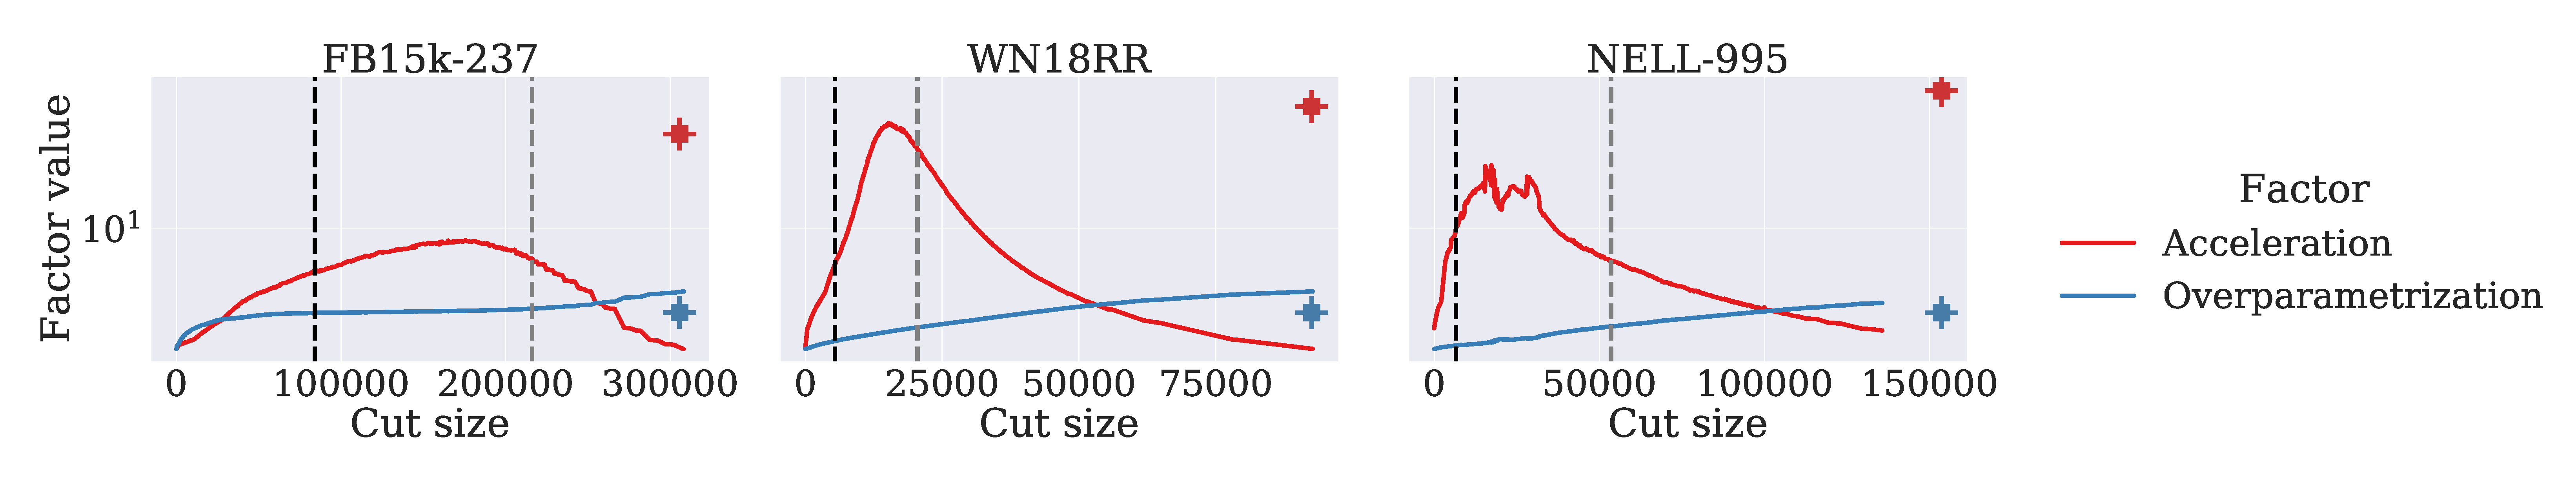
\includegraphics[width=\textwidth]{figures/coins/scalability_leiden_cut_size}
\end{center}
\caption[Dependence of time and memory scalability on the cut size of community partitions obtained by varying the resolution hyperparameter of the Leiden community detection algorithm.]{Dependence of time and memory scalability (acceleration and overparametrization factors) on the cut size (number of inter-community edges) of community partitions obtained by varying the resolution hyperparameter of the Leiden community detection algorithm. Left to right: different datasets. Cut values that yielded optimal balance between scalability and performance for each dataset annotated via black vertical lines. Gray vertical lines denote the cut size values obtained by the METIS algorithm, while the boxes with error bars denote the results from a batch of 100 random uniform community assignments.}
\label{fig:scalability_cut_size}
\end{figure}

Figure~\ref{fig:scalability_modularity} illustrates yet another alternative method to optimize the scalability factors, through optimization of the modularity heuristic utilized by the Leiden algorithm. 

In general, for Leiden, one observes both more acceleration and less overparametrization as modularity increases, however, as the plots display, we found this method to be more unstable than simply traversing the resolution hyperparameter space as before in Figure~\ref{fig:scalability_resolution}. We also note that the METIS algorithm produced slightly higher modularity only for the WN18RR dataset. Random community assignments again, naturally, yield extremal values.

\begin{figure}[H]
\begin{center}
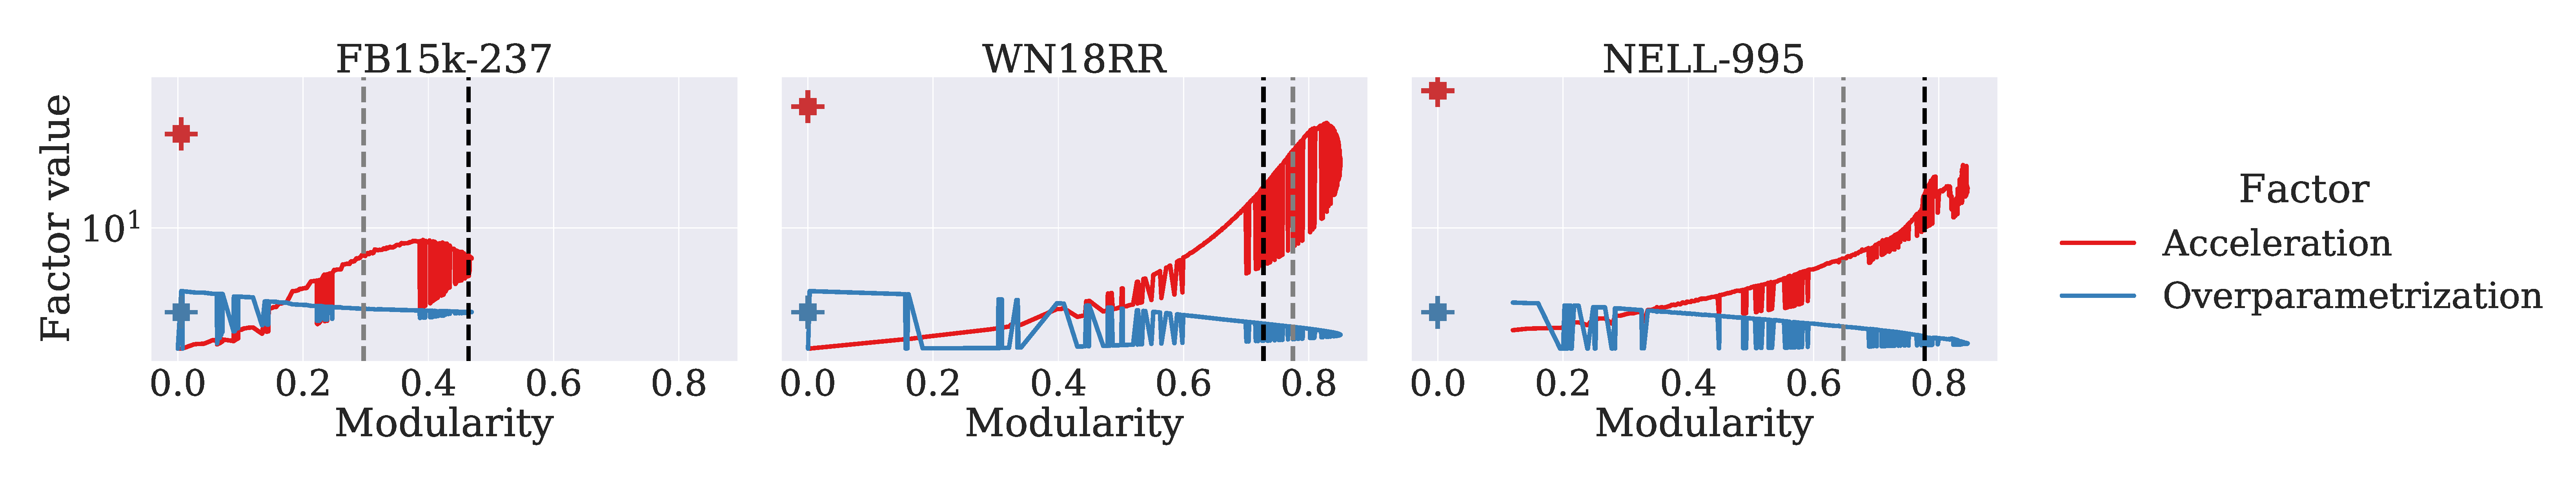
\includegraphics[width=\textwidth]{figures/coins/scalability_leiden_modularity}
\end{center}
\caption[Dependence of time and memory scalability on the value of the modularity heuristic of the Leiden community detection algorithm.]{Dependence of time and memory scalability (acceleration and overparametrization factors) on the value of the modularity heuristic of the Leiden community detection algorithm. Left to right: different datasets. Modularity values that yielded optimal balance between scalability and performance for each dataset annotated via black vertical lines. Gray vertical lines denote the modularity values obtained by the METIS algorithm, while the boxes with error bars denote the results from a batch of 100 random uniform community assignments.}
\label{fig:scalability_modularity}
\end{figure}

\subsection{Performance \& Feasibility}

Table~\ref{tab:performance_query_answering} contains our full query answering metric comparison with the baselines, while Table~\ref{tab:performance_query_answering_2} provides further insight into our query answering performance, after analyzing separately the metrics for each of the two prediction steps. We can observe how well the community Hits@1 score captures the influence of the accuracy in the community prediction on the overall performance. 

Namely, with some quick calculations, one can interestingly note that the overall COINs metric values can be closely approximated as the product of the community Hits@1 and respective scores for the within-community node prediction.

\begin{table}[!ht]
  \caption[All computed query answering metrics.]{All computed query answering metrics (higher is better): comparison of our results with COINs training and evaluation to baselines with equal hyperparameters. Values in bold indicate the superiority of COINs, while underlined values have a relative error lower than 10\%.}
  \label{tab:performance_query_answering}
  \centering
  \begin{adjustbox}{width=\textwidth}   
\begin{tabular}{llllllll}
\toprule
         &           &       &                ComHits@1 &                             Hits@1 &                             Hits@3 &                            Hits@10 &                                MRR \\
Dataset & Algorithm & Value &                          &                                    &                                    &                                    &                                    \\
\midrule
FB15k-237 & TransE & Baseline &                          &                        ${{0.142}}$ &                         ${{0.24}}$ &                        ${{0.369}}$ &                        ${{0.218}}$ \\
         &           & COINs &    ${{0.676}_{\pm 0.0}}$ &            ${{0.078}_{\pm 0.003}}$ &            ${{0.136}_{\pm 0.005}}$ &            ${{0.245}_{\pm 0.007}}$ &            ${{0.132}_{\pm 0.004}}$ \\
         & DistMult & Baseline &                          &                        ${{0.254}}$ &                        ${{0.377}}$ &                        ${{0.527}}$ &                        ${{0.344}}$ \\
         &           & COINs &  ${{0.291}_{\pm 0.045}}$ &            ${{0.038}_{\pm 0.007}}$ &            ${{0.074}_{\pm 0.012}}$ &            ${{0.132}_{\pm 0.012}}$ &            ${{0.068}_{\pm 0.009}}$ \\
         & ComplEx & Baseline &                          &                        ${{0.278}}$ &                        ${{0.404}}$ &                        ${{0.552}}$ &                        ${{0.369}}$ \\
         &           & COINs &  ${{0.975}_{\pm 0.007}}$ &     $\mathbf{{0.333}_{\pm 0.007}}$ &     $\mathbf{{0.477}_{\pm 0.007}}$ &     $\mathbf{{0.626}_{\pm 0.007}}$ &     $\mathbf{{0.431}_{\pm 0.006}}$ \\
         & RotatE & Baseline &                          &                        ${{0.282}}$ &                         ${{0.43}}$ &                        ${{0.584}}$ &                        ${{0.383}}$ \\
         &           & COINs &  ${{0.944}_{\pm 0.001}}$ &     $\mathbf{{0.295}_{\pm 0.003}}$ &  $\underline{{0.416}_{\pm 0.004}}$ &  $\underline{{0.552}_{\pm 0.004}}$ &  $\underline{{0.381}_{\pm 0.003}}$ \\
         & KBGAT & Baseline &                          &                         ${{0.46}}$ &                         ${{0.54}}$ &                        ${{0.626}}$ &                        ${{0.518}}$ \\
         &           & COINs &  ${{0.954}_{\pm 0.005}}$ &            ${{0.163}_{\pm 0.013}}$ &              ${{0.27}_{\pm 0.02}}$ &            ${{0.412}_{\pm 0.024}}$ &            ${{0.245}_{\pm 0.015}}$ \\
         & Query2Box & Baseline &                          &            ${{0.129}_{\pm 0.005}}$ &            ${{0.168}_{\pm 0.002}}$ &              ${{0.2}_{\pm 0.002}}$ &            ${{0.154}_{\pm 0.004}}$ \\
         &           & COINs &  ${{0.721}_{\pm 0.006}}$ &     $\mathbf{{0.186}_{\pm 0.002}}$ &     $\mathbf{{0.289}_{\pm 0.003}}$ &     $\mathbf{{0.402}_{\pm 0.005}}$ &     $\mathbf{{0.261}_{\pm 0.002}}$ \\
\midrule
WN18RR & TransE & Baseline &                          &                        ${{0.019}}$ &                        ${{0.241}}$ &                        ${{0.416}}$ &                         ${{0.16}}$ \\
         &           & COINs &  ${{0.941}_{\pm 0.007}}$ &     $\mathbf{{0.199}_{\pm 0.006}}$ &     $\mathbf{{0.311}_{\pm 0.008}}$ &     $\mathbf{{0.436}_{\pm 0.012}}$ &     $\mathbf{{0.278}_{\pm 0.008}}$ \\
         & DistMult & Baseline &                          &                        ${{0.399}}$ &                        ${{0.452}}$ &                        ${{0.489}}$ &                        ${{0.433}}$ \\
         &           & COINs &  ${{0.997}_{\pm 0.001}}$ &            ${{0.176}_{\pm 0.063}}$ &            ${{0.305}_{\pm 0.086}}$ &            ${{0.423}_{\pm 0.077}}$ &            ${{0.261}_{\pm 0.071}}$ \\
         & ComplEx & Baseline &                          &                        ${{0.426}}$ &                        ${{0.479}}$ &                        ${{0.526}}$ &                        ${{0.462}}$ \\
         &           & COINs &    ${{0.999}_{\pm 0.0}}$ &             ${{0.297}_{\pm 0.02}}$ &            ${{0.394}_{\pm 0.017}}$ &             ${{0.466}_{\pm 0.01}}$ &            ${{0.358}_{\pm 0.018}}$ \\
         & RotatE & Baseline &                          &                        ${{0.442}}$ &                        ${{0.491}}$ &                        ${{0.538}}$ &                        ${{0.476}}$ \\
         &           & COINs &    ${{0.998}_{\pm 0.0}}$ &  $\underline{{0.436}_{\pm 0.001}}$ &      $\mathbf{{0.51}_{\pm 0.003}}$ &     $\mathbf{{0.586}_{\pm 0.004}}$ &     $\mathbf{{0.487}_{\pm 0.001}}$ \\
         & KBGAT & Baseline &                          &                        ${{0.361}}$ &                        ${{0.483}}$ &                        ${{0.581}}$ &                         ${{0.44}}$ \\
         &           & COINs &    ${{0.998}_{\pm 0.0}}$ &            ${{0.274}_{\pm 0.005}}$ &            ${{0.404}_{\pm 0.006}}$ &             ${{0.52}_{\pm 0.006}}$ &            ${{0.359}_{\pm 0.003}}$ \\
         & Query2Box & Baseline &                          &            ${{0.187}_{\pm 0.004}}$ &            ${{0.308}_{\pm 0.001}}$ &            ${{0.385}_{\pm 0.001}}$ &             ${{0.26}_{\pm 0.001}}$ \\
         &           & COINs &  ${{0.958}_{\pm 0.018}}$ &     $\mathbf{{0.218}_{\pm 0.008}}$ &     $\mathbf{{0.382}_{\pm 0.007}}$ &     $\mathbf{{0.524}_{\pm 0.005}}$ &     $\mathbf{{0.323}_{\pm 0.007}}$ \\
\midrule
NELL-995 & TransE & Baseline &                          &                         ${{0.23}}$ &                        ${{0.368}}$ &                        ${{0.448}}$ &                        ${{0.312}}$ \\
         &           & COINs &    ${{0.971}_{\pm 0.0}}$ &             ${{0.15}_{\pm 0.011}}$ &            ${{0.244}_{\pm 0.012}}$ &            ${{0.356}_{\pm 0.019}}$ &            ${{0.218}_{\pm 0.009}}$ \\
         & DistMult & Baseline &                          &                        ${{0.315}}$ &                        ${{0.434}}$ &                        ${{0.555}}$ &                        ${{0.395}}$ \\
         &           & COINs &  ${{0.906}_{\pm 0.033}}$ &            ${{0.062}_{\pm 0.018}}$ &            ${{0.129}_{\pm 0.025}}$ &            ${{0.333}_{\pm 0.013}}$ &            ${{0.127}_{\pm 0.022}}$ \\
         & ComplEx & Baseline &                          &                        ${{0.362}}$ &                        ${{0.538}}$ &                        ${{0.635}}$ &                        ${{0.466}}$ \\
         &           & COINs &  ${{0.996}_{\pm 0.001}}$ &     $\mathbf{{0.364}_{\pm 0.004}}$ &     $\mathbf{{0.548}_{\pm 0.009}}$ &      $\mathbf{{0.66}_{\pm 0.006}}$ &     $\mathbf{{0.472}_{\pm 0.005}}$ \\
         & RotatE & Baseline &                          &                        ${{0.433}}$ &                         ${{0.52}}$ &                        ${{0.562}}$ &                        ${{0.482}}$ \\
         &           & COINs &    ${{0.996}_{\pm 0.0}}$ &            ${{0.304}_{\pm 0.015}}$ &  $\underline{{0.491}_{\pm 0.023}}$ &     $\mathbf{{0.604}_{\pm 0.016}}$ &            ${{0.412}_{\pm 0.018}}$ \\
         & KBGAT & Baseline &                          &                        ${{0.447}}$ &                        ${{0.564}}$ &                        ${{0.695}}$ &                         ${{0.53}}$ \\
         &           & COINs &    ${{0.997}_{\pm 0.0}}$ &  $\underline{{0.436}_{\pm 0.009}}$ &     $\mathbf{{0.617}_{\pm 0.011}}$ &      $\mathbf{{0.73}_{\pm 0.009}}$ &     $\mathbf{{0.543}_{\pm 0.009}}$ \\
         & Query2Box & Baseline &                          &            ${{0.317}_{\pm 0.006}}$ &            ${{0.432}_{\pm 0.002}}$ &             ${{0.49}_{\pm 0.005}}$ &            ${{0.382}_{\pm 0.004}}$ \\
         &           & COINs &  ${{0.967}_{\pm 0.005}}$ &     $\mathbf{{0.348}_{\pm 0.007}}$ &     $\mathbf{{0.499}_{\pm 0.002}}$ &     $\mathbf{{0.602}_{\pm 0.004}}$ &     $\mathbf{{0.443}_{\pm 0.004}}$ \\
\bottomrule
\end{tabular}
  \end{adjustbox}
\end{table}

% \setlength{\LTcapwidth}{\textwidth}
% \begin{longtable}[ht!]{cccccccc}
\begin{table}[!ht]
  \caption[Decomposition of COINs metrics into the overall values and metrics for the second prediction step separately.]{Decomposition of COINs metrics into the overall values shown before and metrics for the second prediction step separately. Values in bold indicate the superiority of COINs compared to the baselines, while underlined values have a relative error lower than 10\%.}
  \label{tab:performance_query_answering_2}%\tabularnewline
  \centering
  \begin{adjustbox}{width=\textwidth}%{totalheight=\textheight-2.6\baselineskip}
\begin{tabular}{llllllll}
\toprule
         &           &      &                ComHits@1 &                             Hits@1 &                             Hits@3 &                            Hits@10 &                                MRR \\
Dataset & Algorithm & Value &                          &                                    &                                    &                                    &                                    \\
\midrule
FB15k-237 & TransE & Overall &    ${{0.676}_{\pm 0.0}}$ &            ${{0.078}_{\pm 0.003}}$ &            ${{0.136}_{\pm 0.005}}$ &            ${{0.245}_{\pm 0.007}}$ &            ${{0.132}_{\pm 0.004}}$ \\
         &           & Node &                          &     $\mathbf{{0.202}_{\pm 0.002}}$ &     $\mathbf{{0.321}_{\pm 0.003}}$ &      $\mathbf{{0.49}_{\pm 0.005}}$ &     $\mathbf{{0.296}_{\pm 0.002}}$ \\
         & DistMult & Overall &  ${{0.291}_{\pm 0.045}}$ &            ${{0.038}_{\pm 0.007}}$ &            ${{0.074}_{\pm 0.012}}$ &            ${{0.132}_{\pm 0.012}}$ &            ${{0.068}_{\pm 0.009}}$ \\
         &           & Node &                          &            ${{0.162}_{\pm 0.009}}$ &            ${{0.301}_{\pm 0.011}}$ &  $\underline{{0.518}_{\pm 0.011}}$ &            ${{0.272}_{\pm 0.009}}$ \\
         & ComplEx & Overall &  ${{0.975}_{\pm 0.007}}$ &     $\mathbf{{0.333}_{\pm 0.007}}$ &     $\mathbf{{0.477}_{\pm 0.007}}$ &     $\mathbf{{0.626}_{\pm 0.007}}$ &     $\mathbf{{0.431}_{\pm 0.006}}$ \\
         &           & Node &                          &     $\mathbf{{0.344}_{\pm 0.008}}$ &     $\mathbf{{0.493}_{\pm 0.009}}$ &      $\mathbf{{0.645}_{\pm 0.01}}$ &     $\mathbf{{0.445}_{\pm 0.008}}$ \\
         & RotatE & Overall &  ${{0.944}_{\pm 0.001}}$ &     $\mathbf{{0.295}_{\pm 0.003}}$ &  $\underline{{0.416}_{\pm 0.004}}$ &  $\underline{{0.552}_{\pm 0.004}}$ &  $\underline{{0.381}_{\pm 0.003}}$ \\
         &           & Node &                          &     $\mathbf{{0.323}_{\pm 0.001}}$ &     $\mathbf{{0.453}_{\pm 0.003}}$ &     $\mathbf{{0.593}_{\pm 0.004}}$ &     $\mathbf{{0.414}_{\pm 0.002}}$ \\
         & KBGAT & Overall &  ${{0.954}_{\pm 0.005}}$ &            ${{0.163}_{\pm 0.013}}$ &              ${{0.27}_{\pm 0.02}}$ &            ${{0.412}_{\pm 0.024}}$ &            ${{0.245}_{\pm 0.015}}$ \\
         &           & Node &                          &            ${{0.173}_{\pm 0.013}}$ &            ${{0.286}_{\pm 0.021}}$ &            ${{0.437}_{\pm 0.024}}$ &             ${{0.26}_{\pm 0.016}}$ \\
         & Query2Box & Overall &  ${{0.721}_{\pm 0.006}}$ &     $\mathbf{{0.186}_{\pm 0.002}}$ &     $\mathbf{{0.289}_{\pm 0.003}}$ &     $\mathbf{{0.402}_{\pm 0.005}}$ &     $\mathbf{{0.261}_{\pm 0.002}}$ \\
         &           & Node &                          &     $\mathbf{{0.283}_{\pm 0.004}}$ &     $\mathbf{{0.411}_{\pm 0.003}}$ &     $\mathbf{{0.547}_{\pm 0.002}}$ &     $\mathbf{{0.373}_{\pm 0.003}}$ \\
\midrule
WN18RR & TransE & Overall &  ${{0.941}_{\pm 0.007}}$ &     $\mathbf{{0.199}_{\pm 0.006}}$ &     $\mathbf{{0.311}_{\pm 0.008}}$ &     $\mathbf{{0.436}_{\pm 0.012}}$ &     $\mathbf{{0.278}_{\pm 0.008}}$ \\
         &           & Node &                          &     $\mathbf{{0.212}_{\pm 0.004}}$ &     $\mathbf{{0.336}_{\pm 0.003}}$ &     $\mathbf{{0.477}_{\pm 0.003}}$ &     $\mathbf{{0.299}_{\pm 0.002}}$ \\
         & DistMult & Overall &  ${{0.997}_{\pm 0.001}}$ &            ${{0.176}_{\pm 0.063}}$ &            ${{0.305}_{\pm 0.086}}$ &            ${{0.423}_{\pm 0.077}}$ &            ${{0.261}_{\pm 0.071}}$ \\
         &           & Node &                          &            ${{0.176}_{\pm 0.063}}$ &            ${{0.305}_{\pm 0.086}}$ &            ${{0.424}_{\pm 0.076}}$ &            ${{0.261}_{\pm 0.071}}$ \\
         & ComplEx & Overall &    ${{0.999}_{\pm 0.0}}$ &             ${{0.297}_{\pm 0.02}}$ &            ${{0.394}_{\pm 0.017}}$ &             ${{0.466}_{\pm 0.01}}$ &            ${{0.358}_{\pm 0.018}}$ \\
         &           & Node &                          &             ${{0.297}_{\pm 0.02}}$ &            ${{0.394}_{\pm 0.017}}$ &             ${{0.467}_{\pm 0.01}}$ &            ${{0.358}_{\pm 0.018}}$ \\
         & RotatE & Overall &    ${{0.998}_{\pm 0.0}}$ &  $\underline{{0.436}_{\pm 0.001}}$ &      $\mathbf{{0.51}_{\pm 0.003}}$ &     $\mathbf{{0.586}_{\pm 0.004}}$ &     $\mathbf{{0.487}_{\pm 0.001}}$ \\
         &           & Node &                          &  $\underline{{0.436}_{\pm 0.001}}$ &      $\mathbf{{0.51}_{\pm 0.003}}$ &     $\mathbf{{0.586}_{\pm 0.004}}$ &     $\mathbf{{0.487}_{\pm 0.001}}$ \\
         & KBGAT & Overall &    ${{0.998}_{\pm 0.0}}$ &            ${{0.274}_{\pm 0.005}}$ &            ${{0.404}_{\pm 0.006}}$ &             ${{0.52}_{\pm 0.006}}$ &            ${{0.359}_{\pm 0.003}}$ \\
         &           & Node &                          &            ${{0.274}_{\pm 0.005}}$ &            ${{0.405}_{\pm 0.006}}$ &             ${{0.52}_{\pm 0.006}}$ &            ${{0.359}_{\pm 0.003}}$ \\
         & Query2Box & Overall &  ${{0.958}_{\pm 0.018}}$ &     $\mathbf{{0.218}_{\pm 0.008}}$ &     $\mathbf{{0.382}_{\pm 0.007}}$ &     $\mathbf{{0.524}_{\pm 0.005}}$ &     $\mathbf{{0.323}_{\pm 0.007}}$ \\
         &           & Node &                          &     $\mathbf{{0.218}_{\pm 0.008}}$ &     $\mathbf{{0.382}_{\pm 0.007}}$ &     $\mathbf{{0.524}_{\pm 0.005}}$ &     $\mathbf{{0.323}_{\pm 0.007}}$ \\
\midrule
NELL-995 & TransE & Overall &    ${{0.971}_{\pm 0.0}}$ &             ${{0.15}_{\pm 0.011}}$ &            ${{0.244}_{\pm 0.012}}$ &            ${{0.356}_{\pm 0.019}}$ &            ${{0.218}_{\pm 0.009}}$ \\
         &           & Node &                          &            ${{0.151}_{\pm 0.011}}$ &            ${{0.247}_{\pm 0.011}}$ &            ${{0.364}_{\pm 0.018}}$ &            ${{0.221}_{\pm 0.009}}$ \\
         & DistMult & Overall &  ${{0.906}_{\pm 0.033}}$ &            ${{0.062}_{\pm 0.018}}$ &            ${{0.129}_{\pm 0.025}}$ &            ${{0.333}_{\pm 0.013}}$ &            ${{0.127}_{\pm 0.022}}$ \\
         &           & Node &                          &            ${{0.077}_{\pm 0.023}}$ &            ${{0.169}_{\pm 0.029}}$ &            ${{0.387}_{\pm 0.008}}$ &            ${{0.159}_{\pm 0.021}}$ \\
         & ComplEx & Overall &  ${{0.996}_{\pm 0.001}}$ &     $\mathbf{{0.364}_{\pm 0.004}}$ &     $\mathbf{{0.548}_{\pm 0.009}}$ &      $\mathbf{{0.66}_{\pm 0.006}}$ &     $\mathbf{{0.472}_{\pm 0.005}}$ \\
         &           & Node &                          &     $\mathbf{{0.367}_{\pm 0.004}}$ &     $\mathbf{{0.551}_{\pm 0.009}}$ &     $\mathbf{{0.664}_{\pm 0.006}}$ &     $\mathbf{{0.475}_{\pm 0.005}}$ \\
         & RotatE & Overall &    ${{0.996}_{\pm 0.0}}$ &            ${{0.304}_{\pm 0.015}}$ &  $\underline{{0.491}_{\pm 0.023}}$ &     $\mathbf{{0.604}_{\pm 0.016}}$ &            ${{0.412}_{\pm 0.018}}$ \\
         &           & Node &                          &            ${{0.305}_{\pm 0.015}}$ &  $\underline{{0.493}_{\pm 0.023}}$ &     $\mathbf{{0.607}_{\pm 0.016}}$ &            ${{0.414}_{\pm 0.018}}$ \\
         & KBGAT & Overall &    ${{0.997}_{\pm 0.0}}$ &  $\underline{{0.436}_{\pm 0.009}}$ &     $\mathbf{{0.617}_{\pm 0.011}}$ &      $\mathbf{{0.73}_{\pm 0.009}}$ &     $\mathbf{{0.543}_{\pm 0.009}}$ \\
         &           & Node &                          &  $\underline{{0.436}_{\pm 0.009}}$ &     $\mathbf{{0.618}_{\pm 0.011}}$ &     $\mathbf{{0.731}_{\pm 0.009}}$ &     $\mathbf{{0.544}_{\pm 0.009}}$ \\
         & Query2Box & Overall &  ${{0.967}_{\pm 0.005}}$ &     $\mathbf{{0.348}_{\pm 0.007}}$ &     $\mathbf{{0.499}_{\pm 0.002}}$ &     $\mathbf{{0.602}_{\pm 0.004}}$ &     $\mathbf{{0.443}_{\pm 0.004}}$ \\
         &           & Node &                          &     $\mathbf{{0.351}_{\pm 0.006}}$ &       $\mathbf{{0.503}_{\pm 0.0}}$ &     $\mathbf{{0.607}_{\pm 0.004}}$ &     $\mathbf{{0.447}_{\pm 0.003}}$ \\
\bottomrule
\end{tabular}
    \end{adjustbox}
% \end{longtable}%
\end{table}%

Figure~\ref{fig:feasibility_statistic} proposes a manner for visually verifying the satisfaction of the condition from Proposition~\ref{proposition:condition_applicability}. In the left plot, we observe how the per-community acceleration and relative error in mean rank metrics influence different values across both algorithms and datasets. We observe that most values lie in the feasibility region, except for the weak performance of COINs-TransE and COINs-DistMult on the FB15k-237 graph. However, as shown in the right plot, where we remove the impact of the community prediction performance and only focus on node MR, we observe that the inequality is now satisfied even for these hardest scenarios.

\begin{figure}[H]
\begin{center}
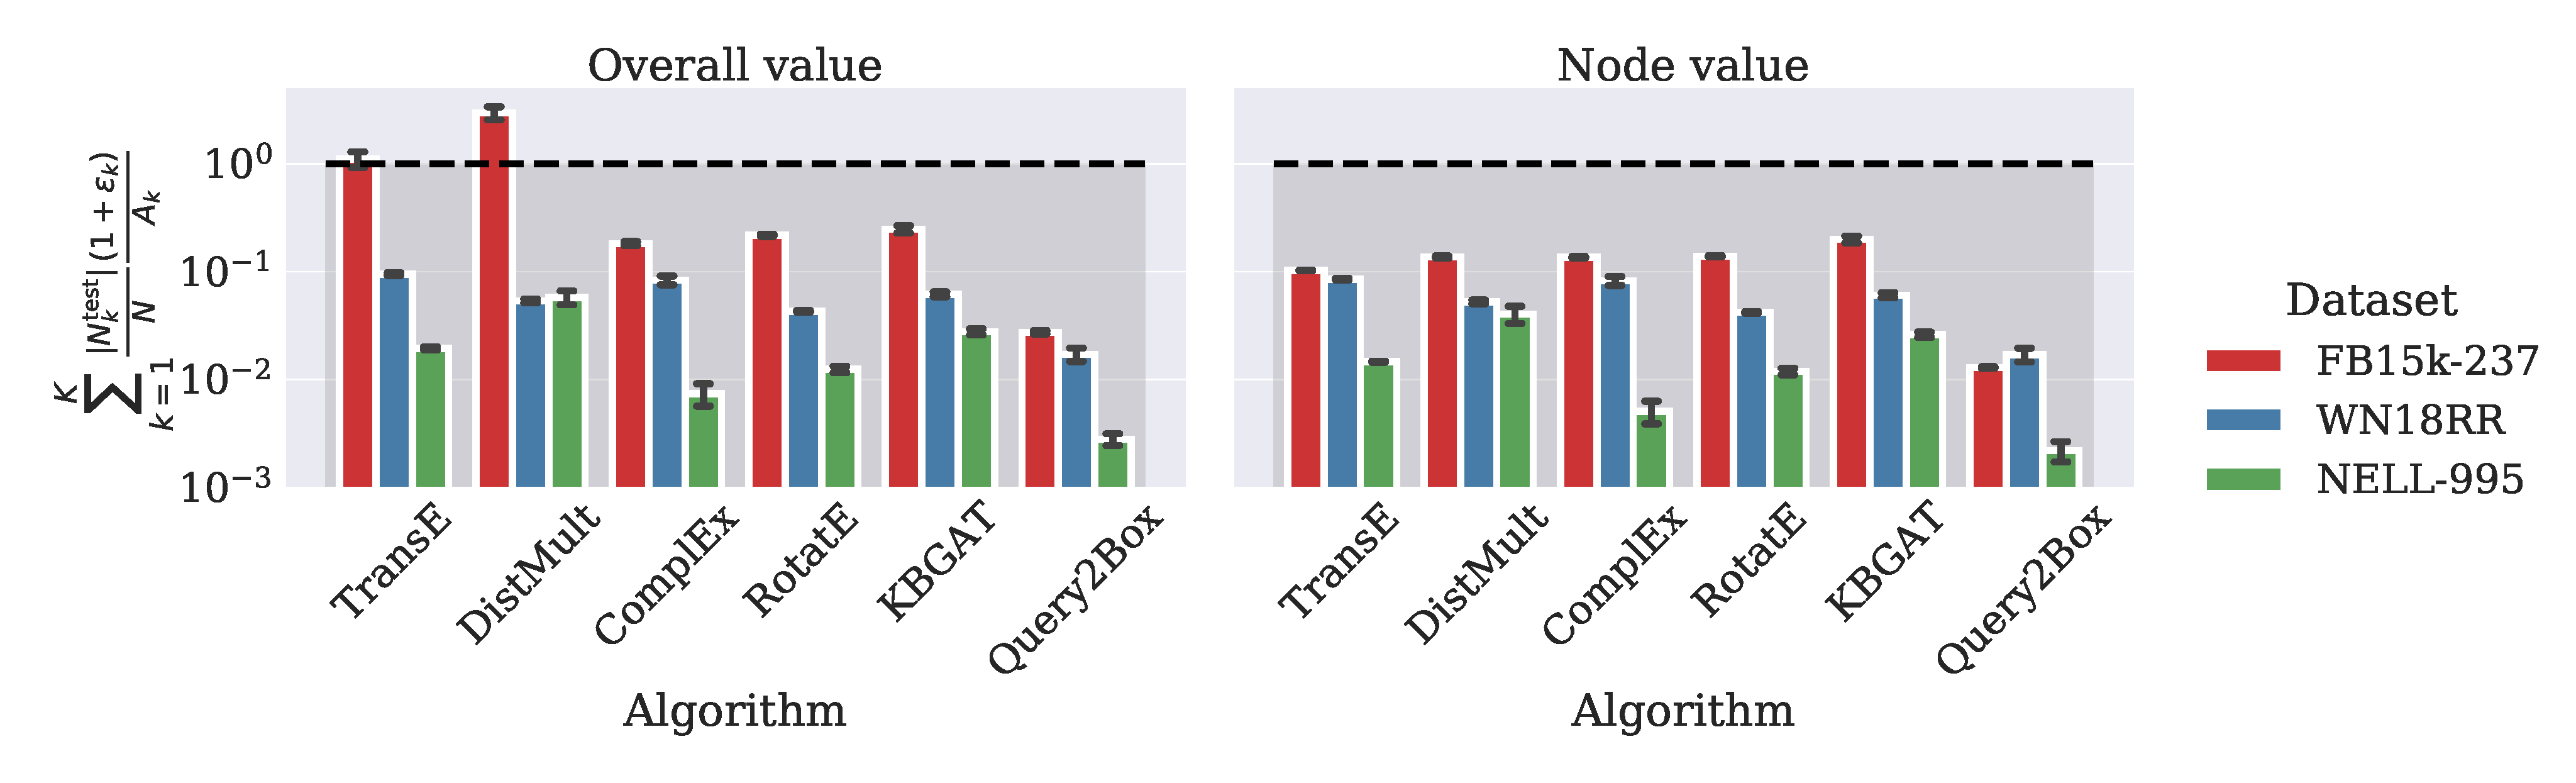
\includegraphics[width=\linewidth]{figures/coins/feasibility_statistic}
\end{center}
\caption[Plot of the values of the COINs feasibility statistic.]{Plot of values of the statistic from Proposition~\ref{proposition:condition_applicability} (lower is better). The feasible region is the one shaded. Left vs. right: statistic values computed from mean ranks after both steps vs. just the second step of COINs.}
\label{fig:feasibility_statistic}
\end{figure}

% \newpage

Figure~\ref{fig:feasibility_trajectories} aims to integrate community assignment validation with model feasibility analysis to explore the tradeoff between achieved community quality (measured by cut size, the count of inter-community edges affecting overparametrization), and the Proposition~\ref{proposition:condition_applicability} statistic (influenced by relative performance error and acceleration). 

To facilitate this tradeoff analysis, we conducted end-to-end training and evaluation for the COINs-RotatE combination on each dataset using various sources of community assignments. Specifically, we varied the Leiden resolution hyperparameter value, considered METIS for another case, and finally, communities assigned uniformly at random.

\begin{figure}[!ht]
\begin{center}
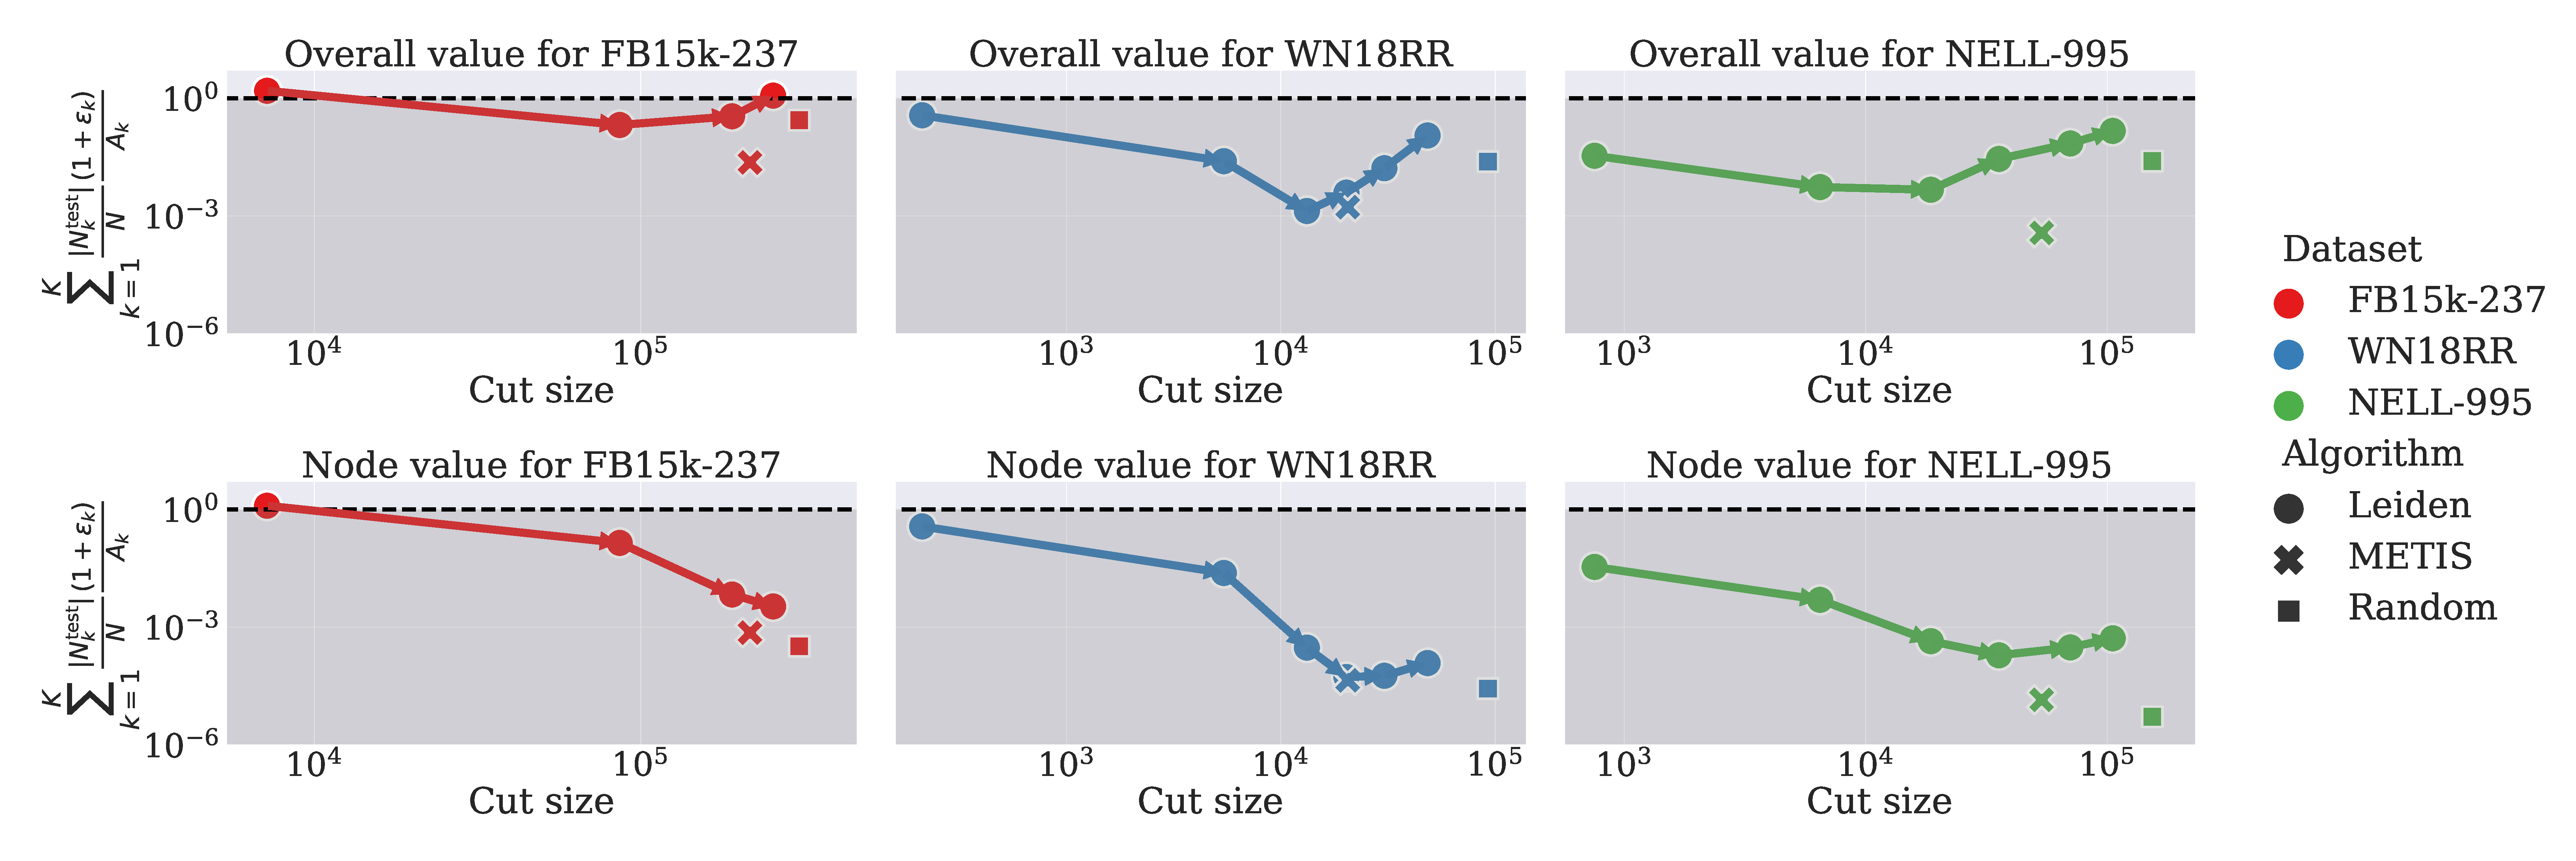
\includegraphics[width=\linewidth]{figures/coins/feasibility_extra}
\end{center}
\caption[Plot of trajectories in the performance-scalability space, for the RotatE algorithm trained and evaluated with different community assignments.]{Plot of trajectories in the performance-scalability space, for the RotatE algorithm trained and evaluated with different community assignments. It is better to have lower cut sizes and lower values of the statistic. The Leiden paths are obtained by varying the resolution hyperparameter, the direction of the arrows indicates an increase of resolution. The feasible region for the statistic from Proposition~\ref{proposition:condition_applicability} is the one shaded. Top vs. bottom: statistic values computed from mean ranks after both steps vs. just the second step of COINs. Left to right: different datasets.}
\label{fig:feasibility_trajectories}
\end{figure}

Leiden trajectories for all datasets possess a critical point in the statistic, revealing the existence of an optimal trade-off between relative error and acceleration. Cut sizes, however, exhibit a simple increase as Leiden resolution increases. For FB15k-237, we cross the feasibility boundary of Proposition~\ref{proposition:condition_applicability} by adjusting the resolution. 

When focusing solely on performance in the second prediction step, relative error improves more rapidly with Leiden resolution, resulting in lower values for the statistic. It is noteworthy that this is anticipated, as higher Leiden resolution implies smaller communities, leading to fewer possible query answers. 

Finally, we affirm that although METIS and random communities may yield higher speed-ups, numerous Leiden community assignments achieve comparable performance with equally significant speed-ups but considerably smaller cut sizes, thereby reducing the number of model parameters.

Table~\ref{tab:performance_link_prediction} contains all of our results on the link prediction task. We do not possess baselines for these results due to the limited scope of the related work, which focuses only on an evaluation of the query answering task. Thus, we cannot perform a similar comparison as before. Regardless, the relative ordering of the metric values across settings is consistent with the query answering performance discussed previously.

\begin{table}[ht!]
  \caption[All computed link prediction metrics.]{All computed link prediction metrics (higher is better), with community prediction metrics also given separately.}
  \label{tab:performance_link_prediction}
  \centering
    \begin{adjustbox}{width=\textwidth}%{totalheight=\textheight-2.6\baselineskip}
\begin{tabular}{lllllll}
\toprule
         &           &         &                 Accuracy &                       F1 &                  ROC-AUC &                       AP \\
Dataset & Algorithm & Value &                          &                          &                          &                          \\
\midrule
FB15k-237 & TransE & Community &    ${{0.946}_{\pm 0.0}}$ &    ${{0.941}_{\pm 0.0}}$ &    ${{0.964}_{\pm 0.0}}$ &  ${{0.812}_{\pm 0.005}}$ \\
         &           & Overall &  ${{0.895}_{\pm 0.001}}$ &  ${{0.896}_{\pm 0.001}}$ &     ${{0.94}_{\pm 0.0}}$ &  ${{0.727}_{\pm 0.003}}$ \\
         & DistMult & Community &  ${{0.864}_{\pm 0.007}}$ &  ${{0.877}_{\pm 0.006}}$ &   ${{0.97}_{\pm 0.004}}$ &  ${{0.861}_{\pm 0.016}}$ \\
         &           & Overall &  ${{0.908}_{\pm 0.002}}$ &  ${{0.912}_{\pm 0.001}}$ &   ${{0.95}_{\pm 0.001}}$ &  ${{0.841}_{\pm 0.005}}$ \\
         & ComplEx & Community &    ${{0.997}_{\pm 0.0}}$ &    ${{0.997}_{\pm 0.0}}$ &    ${{0.998}_{\pm 0.0}}$ &    ${{0.996}_{\pm 0.0}}$ \\
         &           & Overall &  ${{0.938}_{\pm 0.004}}$ &  ${{0.938}_{\pm 0.003}}$ &    ${{0.968}_{\pm 0.0}}$ &    ${{0.9}_{\pm 0.002}}$ \\
         & RotatE & Community &  ${{0.988}_{\pm 0.001}}$ &  ${{0.989}_{\pm 0.001}}$ &    ${{0.998}_{\pm 0.0}}$ &    ${{0.995}_{\pm 0.0}}$ \\
         &           & Overall &  ${{0.925}_{\pm 0.001}}$ &  ${{0.922}_{\pm 0.001}}$ &   ${{0.96}_{\pm 0.001}}$ &  ${{0.853}_{\pm 0.003}}$ \\
         & KBGAT & Community &    ${{0.995}_{\pm 0.0}}$ &    ${{0.995}_{\pm 0.0}}$ &    ${{0.999}_{\pm 0.0}}$ &    ${{0.998}_{\pm 0.0}}$ \\
         &           & Overall &  ${{0.884}_{\pm 0.005}}$ &  ${{0.858}_{\pm 0.008}}$ &  ${{0.935}_{\pm 0.007}}$ &  ${{0.789}_{\pm 0.019}}$ \\
         & Query2Box & Community &  ${{0.835}_{\pm 0.003}}$ &  ${{0.762}_{\pm 0.007}}$ &    ${{0.992}_{\pm 0.0}}$ &    ${{0.977}_{\pm 0.0}}$ \\
         &           & Overall &    ${{0.833}_{\pm 0.0}}$ &    ${{0.758}_{\pm 0.0}}$ &  ${{0.918}_{\pm 0.001}}$ &  ${{0.747}_{\pm 0.004}}$ \\
\midrule
WN18RR & TransE & Community &    ${{0.989}_{\pm 0.0}}$ &    ${{0.989}_{\pm 0.0}}$ &    ${{0.986}_{\pm 0.0}}$ &  ${{0.963}_{\pm 0.006}}$ \\
         &           & Overall &  ${{0.905}_{\pm 0.002}}$ &  ${{0.904}_{\pm 0.001}}$ &  ${{0.923}_{\pm 0.001}}$ &  ${{0.798}_{\pm 0.005}}$ \\
         & DistMult & Community &  ${{0.882}_{\pm 0.003}}$ &  ${{0.893}_{\pm 0.002}}$ &    ${{0.999}_{\pm 0.0}}$ &    ${{0.998}_{\pm 0.0}}$ \\
         &           & Overall &   ${{0.92}_{\pm 0.002}}$ &  ${{0.913}_{\pm 0.002}}$ &   ${{0.86}_{\pm 0.003}}$ &  ${{0.752}_{\pm 0.005}}$ \\
         & ComplEx & Community &      ${{1.0}_{\pm 0.0}}$ &      ${{1.0}_{\pm 0.0}}$ &      ${{1.0}_{\pm 0.0}}$ &      ${{1.0}_{\pm 0.0}}$ \\
         &           & Overall &  ${{0.925}_{\pm 0.001}}$ &  ${{0.917}_{\pm 0.001}}$ &  ${{0.912}_{\pm 0.001}}$ &  ${{0.814}_{\pm 0.001}}$ \\
         & RotatE & Community &    ${{0.997}_{\pm 0.0}}$ &    ${{0.997}_{\pm 0.0}}$ &    ${{0.999}_{\pm 0.0}}$ &    ${{0.999}_{\pm 0.0}}$ \\
         &           & Overall &    ${{0.912}_{\pm 0.0}}$ &      ${{0.9}_{\pm 0.0}}$ &  ${{0.949}_{\pm 0.001}}$ &  ${{0.871}_{\pm 0.001}}$ \\
         & KBGAT & Community &    ${{0.999}_{\pm 0.0}}$ &    ${{0.999}_{\pm 0.0}}$ &      ${{1.0}_{\pm 0.0}}$ &    ${{0.999}_{\pm 0.0}}$ \\
         &           & Overall &  ${{0.917}_{\pm 0.002}}$ &  ${{0.906}_{\pm 0.003}}$ &  ${{0.936}_{\pm 0.003}}$ &   ${{0.86}_{\pm 0.003}}$ \\
         & Query2Box & Community &  ${{0.837}_{\pm 0.003}}$ &  ${{0.766}_{\pm 0.007}}$ &    ${{0.999}_{\pm 0.0}}$ &    ${{0.999}_{\pm 0.0}}$ \\
         &           & Overall &    ${{0.833}_{\pm 0.0}}$ &    ${{0.758}_{\pm 0.0}}$ &  ${{0.888}_{\pm 0.003}}$ &   ${{0.68}_{\pm 0.008}}$ \\
\midrule
NELL-995 & TransE & Community &    ${{0.995}_{\pm 0.0}}$ &    ${{0.995}_{\pm 0.0}}$ &  ${{0.992}_{\pm 0.002}}$ &  ${{0.982}_{\pm 0.002}}$ \\
         &           & Overall &  ${{0.932}_{\pm 0.001}}$ &  ${{0.933}_{\pm 0.001}}$ &  ${{0.963}_{\pm 0.001}}$ &  ${{0.818}_{\pm 0.009}}$ \\
         & DistMult & Community &   ${{0.95}_{\pm 0.003}}$ &  ${{0.952}_{\pm 0.003}}$ &  ${{0.996}_{\pm 0.001}}$ &  ${{0.978}_{\pm 0.007}}$ \\
         &           & Overall &  ${{0.943}_{\pm 0.002}}$ &  ${{0.943}_{\pm 0.002}}$ &  ${{0.931}_{\pm 0.002}}$ &  ${{0.836}_{\pm 0.006}}$ \\
         & ComplEx & Community &    ${{0.999}_{\pm 0.0}}$ &    ${{0.999}_{\pm 0.0}}$ &    ${{0.999}_{\pm 0.0}}$ &    ${{0.999}_{\pm 0.0}}$ \\
         &           & Overall &  ${{0.968}_{\pm 0.001}}$ &  ${{0.968}_{\pm 0.001}}$ &     ${{0.99}_{\pm 0.0}}$ &  ${{0.961}_{\pm 0.002}}$ \\
         & RotatE & Community &  ${{0.993}_{\pm 0.001}}$ &  ${{0.993}_{\pm 0.001}}$ &      ${{1.0}_{\pm 0.0}}$ &    ${{0.999}_{\pm 0.0}}$ \\
         &           & Overall &  ${{0.947}_{\pm 0.004}}$ &  ${{0.945}_{\pm 0.004}}$ &  ${{0.977}_{\pm 0.001}}$ &  ${{0.885}_{\pm 0.009}}$ \\
         & KBGAT & Community &    ${{0.999}_{\pm 0.0}}$ &    ${{0.999}_{\pm 0.0}}$ &      ${{1.0}_{\pm 0.0}}$ &      ${{1.0}_{\pm 0.0}}$ \\
         &           & Overall &  ${{0.944}_{\pm 0.005}}$ &  ${{0.939}_{\pm 0.006}}$ &  ${{0.985}_{\pm 0.001}}$ &  ${{0.957}_{\pm 0.002}}$ \\
         & Query2Box & Community &  ${{0.834}_{\pm 0.001}}$ &  ${{0.759}_{\pm 0.002}}$ &    ${{0.999}_{\pm 0.0}}$ &  ${{0.998}_{\pm 0.001}}$ \\
         &           & Overall &    ${{0.833}_{\pm 0.0}}$ &    ${{0.758}_{\pm 0.0}}$ &  ${{0.963}_{\pm 0.002}}$ &  ${{0.882}_{\pm 0.005}}$ \\
\bottomrule
\end{tabular}
  \end{adjustbox}
\end{table}%

% Figure~\ref{fig:feasibility_trajectories} is our most detailed experiment, with the goal of merging together the validation of community assignments with the analysis of model feasibility, to investigate the tradeoff between achieved community quality, relative error in performance and acceleration/overparametrization. To facilitate this, for each dataset we end-to-end trained and evaluated the COINs-RotatE combination (as our most successful) with different sources of community assignments. Namely, we searched the region around the optimal value for the Leiden resolution hyperparameter to obtain worse communities, replaced Leiden with METIS for another case, and for a final run picked one random uniform community assignment.

% As in Figures~\ref{fig:scalability_resolution} and~\ref{fig:scalability_cut_size}, we observe that the Leiden trajectories for all datasets have a critical point with an optimal trade-off between relative error and acceleration. We note that overall relative error, although unstable w.r.t. Leiden resolution, does not vary greatly and the main differences seem to lie in the acceleration values (although for FB15k-237 we manage to enter and exit the feasibility region by changing resolution). On the other hand, when considering only the performance in the second prediction step, relative error improves with Leiden resolution much faster. Note that, however, this is to be expected, as greater Leiden resolution implies smaller communities and thus, fewer possible answers to queries. We confirm again that overparametrization simply increases with greater resolution values and dominates the trajectory direction in the overall performance case. Thus, we confirm again that although the METIS and random communities might yield higher speed-ups, there are a lot of Leiden community assignments resulting in similar performance, and equally significant speed-ups but with significantly fewer parameters. 

% \begin{figure}[ht!]
% \begin{center}
% \includegraphics[width=\textwidth]{figures/feasibility_rebuttals}
% \includegraphics[width=\textwidth]{figures/feasibility_rebuttals_2}
% \end{center}
% \caption{Plot of trajectories in the performance-scalability space, for the RotatE algorithm trained and evaluated with different community assignments. The Leiden paths are obtained by varying the resolution hyperparameter, the direction of the arrows indicates an increase of resolution. The feasible region for acceleration (Proposition~\ref{proposition:condition_applicability}) is the one shaded. Odd vs. even rows: COINs metric values after both steps vs. just the second step. Top two vs. bottom two rows: acceleration vs. overparametrization space.}
% \label{fig:feasibility_trajectories}
% \end{figure}



\subsection{Stability \& Convergence}

The convergence plots in Figure~\ref{fig:convergence} support our decision to model the final aggregate COINs loss value as the linear combination of the community and node terms. From the convergence lines, one can observe that the community and node iterates seem to converge at equal rates in both training and validation data. As such, the aggregate COINs loss function can be a simple average of the two terms without affecting convergence.

\begin{figure}[!ht]
\begin{center}
\includegraphics[width=\textwidth]{figures/coins/convergence}
\end{center}
\caption[Plots of contrastive loss convergence over time.]{Plots of contrastive loss convergence over time, with the decomposition of the final COINs loss into the two constituent community and node loss terms. Top vs. bottom: training vs. validation loss. Left to right: the different COINs-integrated algorithms. Error bands show standard deviation across datasets.}
\label{fig:convergence}
\end{figure}

% \clearpage

\section{Practical speed-ups}
All of the discussion on the acceleration benefits of COINs so far only concerned the reduction in computational complexity, i.e. how much fewer embedding operations are performed during evaluation. For completeness, we also estimated the speed-up one would observe in practice, i.e. the reduction in total CPU seconds of the evaluation process compared to the baseline. 

From the visualization of these results in Figure~\ref{fig:acceleration_wall} we can deduce that even w.r.t. wall time COINs always provides at least around 2 times speed-up, while the time-memory trade-off employed by NodePiece and EARL is also evident. The slow-down factors incurred by these methods are too great to justify the comparatively smaller memory-usage reduction factors. However, due to high variance in the experiment conditions during measurement, as well as differences in the practical complexity of the embedding algorithm implementations, these acceleration numerics are inconsistent across different settings and with large error bars. For such reasons, we relied mainly on the more reliable measurements of computation steps.

\begin{figure}[ht!]
\begin{center}
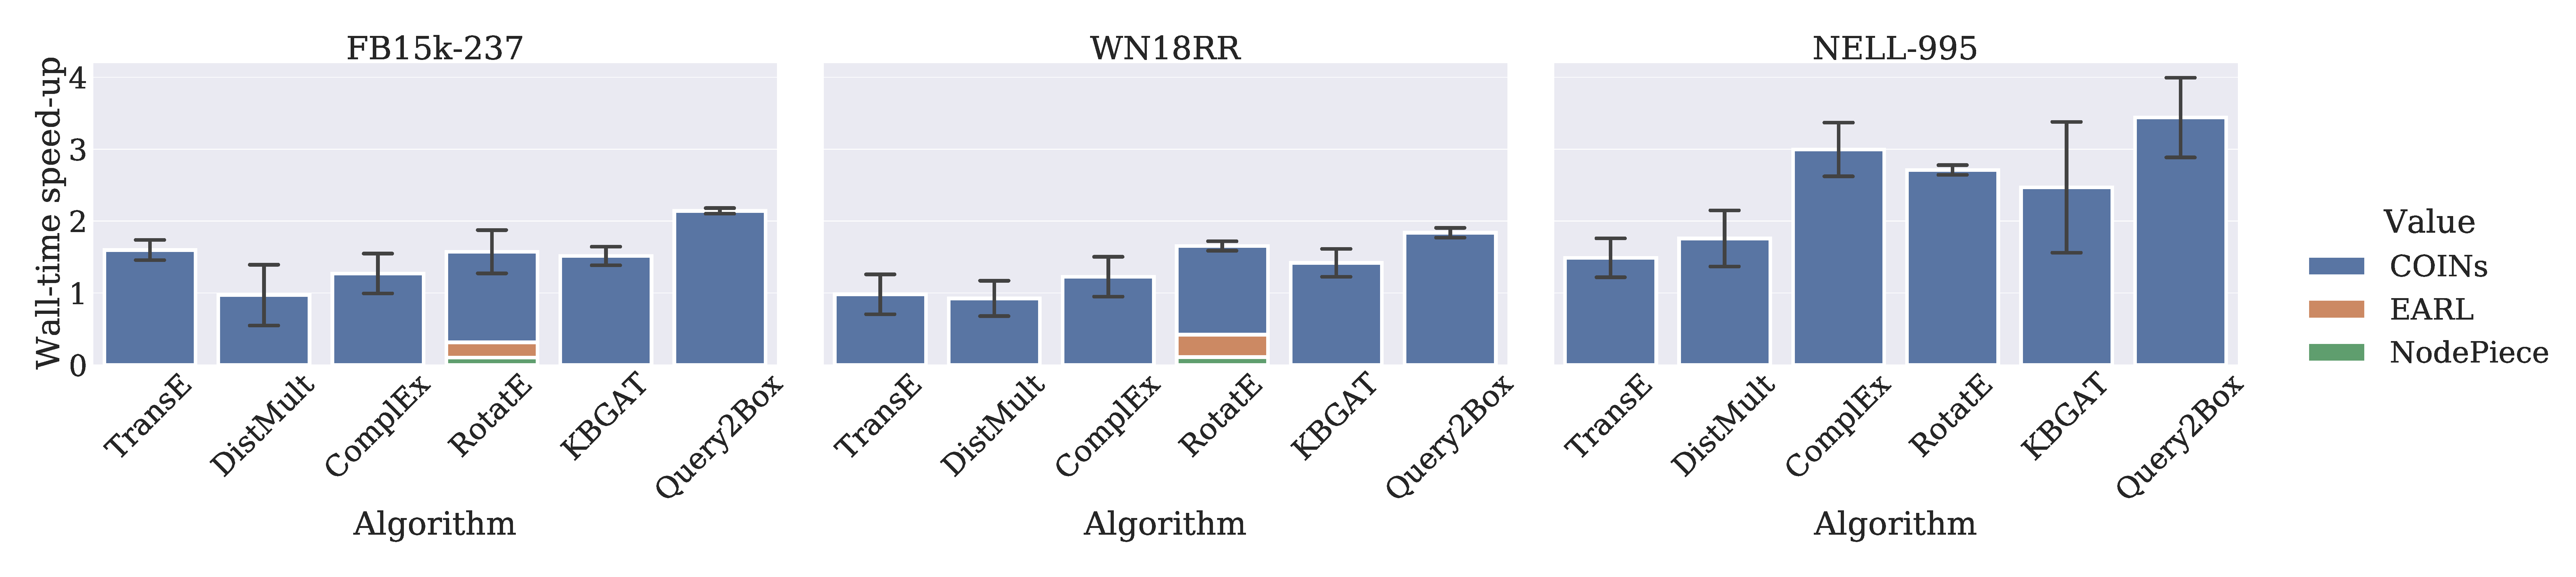
\includegraphics[width=\textwidth]{figures/coins/acceleration_wall}
\end{center}
\caption[CPU time speed-up thanks to COINs.]{Per-algorithm evaluation CPU time speed-up thanks to COINs, averaged across multiple seeds. Left to right: different datasets.}
\label{fig:acceleration_wall}
\end{figure}

\section{Implementation details}
\label{sec:appendix_implementation}

The entire implementation was performed in the Python 3.6 programming language. The Pandas library~\cite{mckinney_data_2010} was helpful with its efficient preprocessing operations on tabular data. The iGraph library~\cite{csardi_igraph_2005} was utilized for the implementation of most of the graph analysis and preprocessing steps, including executing the Leiden algorithm. For METIS, the official software implementation~\cite{karypis_metis_1997} was invoked through a Python wrapper. 

The entire model architecture (along with integration code for the publicly available implementations of the external embedders), training, and evaluation, were implemented using the PyTorch deep learning framework~\cite{paszke_pytorch_2019} and the extension framework for graph neural network learning PyTorch Geometric~\cite{fey_fast_2019}. 

All code was executed on a single machine with the following specifications:
\begin{itemize}
    % \item Intel\textsuperscript{\textregistered} Xeon\textsuperscript{\textregistered} Gold 5118 12-core CPU @ 2.30GHz;
    % \item NVIDIA Tesla P100-PCIE-16GB GPU;
    % \item 64GB RAM.
    \item AMD EPYC\textsuperscript{\texttrademark} 7742 64-core CPU @ 2.25GHz;
    \item NVIDIA A100-SXM4-40GB GPU;
    \item 1.0TB RAM. 
\end{itemize}

% To facilitate reproducibility, our full code implementation is available at: \\
% \url{https://github.com/LIONS-EPFL/coins-ict-innovations-2025}.

% \section{Appendix}
% Any possible appendices should be placed after bibliographies.
% If your paper has appendices, please submit the appendices together with the main body of the paper.
% There will be no separate supplementary material submission.
% The main text should be self-contained; reviewers are not obliged to look at the appendices when writing their review comments.


% \section{First Section}
% \subsection{A Subsection Sample}
% Please note that the first paragraph of a section or subsection is
% not indented. The first paragraph that follows a table, figure,
% equation etc. does not need an indent, either.

% Subsequent paragraphs, however, are indented.

% \subsubsection{Sample Heading (Third Level)} Only two levels of
% headings should be numbered. Lower level headings remain unnumbered;
% they are formatted as run-in headings.

% \paragraph{Sample Heading (Fourth Level)}
% The contribution should contain no more than four levels of
% headings. Table~\ref{tab1} gives a summary of all heading levels.

% \begin{table}
% \caption{Table captions should be placed above the
% tables.}\label{tab1}
% \begin{tabular}{lll}
% \hline
% Heading level &  Example & Font size and style\\
% \hline
% Title (centered) &  {\Large\bfseries Lecture Notes} & 14 point, bold\\
% 1st-level heading &  {\large\bfseries 1 Introduction} & 12 point, bold\\
% 2nd-level heading & {\bfseries 2.1 Printing Area} & 10 point, bold\\
% 3rd-level heading & {\bfseries Run-in Heading in Bold.} Text follows & 10 point, bold\\
% 4th-level heading & {\itshape Lowest Level Heading.} Text follows & 10 point, italic\\
% \hline
% \end{tabular}
% \end{table}


% \noindent Displayed equations are centered and set on a separate
% line.
% \begin{equation}
% x + y = z
% \end{equation}
% Please try to avoid rasterized images for line-art diagrams and
% schemas. Whenever possible, use vector graphics instead (see
% Fig.~\ref{fig1}).

% \begin{figure}
% \includegraphics[width=\textwidth]{fig1.eps}
% \caption{A figure caption is always placed below the illustration.
% Please note that short captions are centered, while long ones are
% justified by the macro package automatically.} \label{fig1}
% \end{figure}

% \begin{theorem}
% This is a sample theorem. The run-in heading is set in bold, while
% the following text appears in italics. Definitions, lemmas,
% propositions, and corollaries are styled the same way.
% \end{theorem}
% %
% % the environments 'definition', 'lemma', 'proposition', 'corollary',
% % 'remark', and 'example' are defined in the LLNCS documentclass as well.
% %
% \begin{proof}
% Proofs, examples, and remarks have the initial word in italics,
% while the following text appears in normal font.
% \end{proof}
% For citations of references, we prefer the use of square brackets
% and consecutive numbers. Citations using labels or the author/year
% convention are also acceptable. The following bibliography provides
% a sample reference list with entries for journal
% articles~\cite{ref_article1}, an LNCS chapter~\cite{ref_lncs1}, a
% book~\cite{ref_book1}, proceedings without editors~\cite{ref_proc1},
% and a homepage~\cite{ref_url1}. Multiple citations are grouped
% \cite{ref_article1,ref_lncs1,ref_book1},
% \cite{ref_article1,ref_book1,ref_proc1,ref_url1}.

\chapter{Appendix for HiGenDiff}

\section{Proofs}
\label{sec:appendix_higendiff_theory}

\begin{proof}[Proposition~\ref{proposition:complexity_higendiff}]
Let $\offf{c^{\of{L}}_k}_{k=1}^{n^{\of{L+1}}}$ be the sizes of the communities imposed by $M^{\of{L}}$, i.e., $\forall k, c^{\of{L}}_k=\sum_{i=1}^{n^{\of{L}}}{M^{\of{L}}_{k,i}}$. Then the worst-case cost of one diffusion step of HiGenDiff for a given adjacency matrix $A^{\of{L}}$ will be thus ${n^{\of{L+1}}}^2 + \sum_{j=1}^{n^{\of{L+1}}}\sum_{k=1}^{n^{\of{L+1}}}{c^{\of{L}}_j c^{\of{L}}_k \bar{A}_{j,k}^{\of{L+1}}}$. This is because we need to sample all the edges of the parent graph and then sample all communities and the bipartites that should exist, according to the parent level's adjacency. Since all the above quantities are random variables, under the i.i.d. Bernoulli assumption the expectation yields:
\begin{align}
    \begin{split}
        \mathbb{E}\off{{n^{\of{L+1}}}^2 + \sum_{j=1}^{n^{\of{L+1}}}\sum_{k=1}^{n^{\of{L+1}}}{c^{\of{L}}_j c^{\of{L}}_k \bar{A}_{j,k}^{\of{L+1}}}} 
        &= \mathbb{E}\off{{n^{\of{L+1}}}^2}+\sum_{j=1}^{n^{\of{L+1}}}\sum_{k=1}^{n^{\of{L+1}}}{\mathbb{E}\off{c^{\of{L}}_j c^{\of{L}}_k} \mathbb{E}\off{\bar{A}_{j,k}^{\of{L+1}}}} \\
        &= \mathbb{E}\off{{n^{\of{L+1}}}^2}+p\sum_{j=1}^{n^{\of{L+1}}}\sum_{k=1}^{n^{\of{L+1}}}{\of{\mathrm{Cov}\off{c^{\of{L}}_j,c^{\of{L}}_k}+\mathbb{E}\off{c^{\of{L}}_j}\mathbb{E}\off{c^{\of{L}}_k}}} \\
        &= \mathbb{E}\off{{n^{\of{L+1}}}^2}+p\of{\mathrm{Cov}\off{\sum_{j=1}^{n^{\of{L+1}}}{c^{\of{L}}_j},\sum_{k=1}^{n^{\of{L+1}}}{c^{\of{L}}_k}}+\mathbb{E}\off{\sum_{k=1}^{n^{\of{L+1}}}{c^{\of{L}}_k}}^2}\\
         &= \mathbb{E}\off{{n^{\of{L+1}}}^2} +p \of{\mathbb{V}\off{n^{\of{L}}}+\mathbb{E}\off{n^{\of{L}}}^2} \\
          &= \mathbb{E}\off{{n^{\of{L+1}}}^2} + p\mathbb{E}\off{{n^{\of{L}}}^2}
    \end{split}
\end{align}
For the upper bound, note that always $p \leq 1$ and $n^{\of{L+1}} \leq n^{\of{L}}$.

For the lower bound, we know that $p \geq \frac{1}{n^{\of{L+1}}}$, as in the best case, there will not be a single bipartite to generate, but we always have to sample the communities (the self-loops in the parent). Thus taking the expectation of $p$ w.r.t. $n^{\of{L}}$ implies: $\mathbb{E}\off{{n^{\of{L+1}}}^2} +p\mathbb{E}\off{{n^{\of{L}}}^2} \geq \mathbb{E}\off{{n^{\of{L+1}}}^2 + \frac{{n^{\of{L}}}^2}{n^{\of{L+1}}}}$. Similar to the proof of Proposition \ref{proposition:complexity_distributed}, we find that the minimum of the function $f\of{K}=K^2+\frac{\abs{V}}{K}$ is $\frac{3}{2}\sqrt[3]{2\abs{V}^2}$ and is achieved when $K=\frac{1}{2}\sqrt[3]{4\abs{V}}$. Plugging in $\abs{V}={n^{\of{L}}}^2$ and $K=n^{\of{L+1}}$ yields the result.
\end{proof}

\section{Detailed results}
\label{sec:appendix_higendiff_results}

\begin{table}[H]
    \centering
\caption[All MMD metrics for HiGenDiff.]{All MMD metrics (lower is better) for HiGenDiff of the model ablation experiments for each dataset.}
\label{tab:higendiff_full}
\begin{adjustbox}{width=\textwidth}
    \begin{tabular}{lllrrrr}
\toprule
 &  &  & Degree MMD & Cluster MMD & Orbit MMD & Spectral MMD \\
Dataset & Model & Bucketized &  &  &  &  \\
\midrule
\multirow[t]{5}{*}{enzyme} & Simple & No & 0.002 & 0.018 & 0.046 & 0.008 \\
% \cline{2-7}
 & \multirow[t]{2}{*}{Integer} & No & 0.007 & 0.019 & 0.048 & 0.01 \\
 &  & Yes & 0.004 & 0.016 & 0.025 & 0.005 \\
% \cline{2-7}
 & \multirow[t]{2}{*}{Ordinal} & No & 0.007 & 0.018 & 0.034 & 0.007 \\
 &  & Yes & 0.004 & 0.019 & 0.043 & 0.008 \\
% \cline{1-7} \cline{2-7}
\midrule
\multirow[t]{5}{*}{SBM} & Simple & No & 0.002 & 0.03 & 0.044 & 0.004 \\
% \cline{2-7}
 & \multirow[t]{2}{*}{Integer} & No & 0.001 & 0.028 & 0.047 & 0.004 \\
 &  & Yes & 0.001 & 0.027 & 0.04 & 0.004 \\
% \cline{2-7}
 & \multirow[t]{2}{*}{Ordinal} & No & 0.001 & 0.029 & 0.046 & 0.004 \\
 &  & Yes & 0.001 & 0.03 & 0.068 & 0.005 \\
% \cline{1-7} \cline{2-7}
\midrule
\multirow[t]{5}{*}{Ego2} & Simple & No & 0.002 & 0.06 & 0.036 & 0.005 \\
% \cline{2-7}
 & \multirow[t]{2}{*}{Integer} & No & 0.002 & 0.065 & 0.033 & 0.003 \\
 &  & Yes & 0.002 & 0.055 & 0.053 & 0.007 \\
% \cline{2-7}
 & \multirow[t]{2}{*}{Ordinal} & No & 0.011 & 0.064 & 0.035 & 0.02 \\
 &  & Yes & 0.002 & 0.059 & 0.042 & 0.004 \\
% \cline{1-7} \cline{2-7}
\midrule
\multirow[t]{5}{*}{DD2} & Simple & No & 0.004 & 0.08 & 0.024 & 0.005 \\
% \cline{2-7}
 & \multirow[t]{2}{*}{Integer} & No & 0.009 & 0.092 & 0.05 & 0.007 \\
 &  & Yes & 0.013 & 0.109 & 0.035 & 0.008 \\
% \cline{2-7}
 & \multirow[t]{2}{*}{Ordinal} & No & 0.002 & 0.072 & 0.112 & 0.007 \\
 &  & Yes & 0.008 & 0.09 & 0.031 & 0.007 \\
% \cline{1-7} \cline{2-7}
\midrule
\multirow[t]{5}{*}{RoC} & Simple & No & 0.003 & 0.218 & 0.002 & 0.027 \\
% \cline{2-7}
 & \multirow[t]{2}{*}{Integer} & No & 0.013 & 0.312 & 0.014 & 0.044 \\
 &  & Yes & 0.008 & 0.266 & 0.018 & 0.039 \\
% \cline{2-7}
 & \multirow[t]{2}{*}{Ordinal} & No & 0.015 & 0.297 & 0.029 & 0.044 \\
 &  & Yes & 0.01 & 0.298 & 0.019 & 0.041 \\
% \cline{1-7} \cline{2-7}
\midrule
\multirow[t]{5}{*}{LFR} & Simple & No & 0.022 & 0.214 & 0.12 & 0.004 \\
% \cline{2-7}
 & \multirow[t]{2}{*}{Integer} & No & 0.103 & 0.309 & 0.448 & 0.055 \\
 &  & Yes & 0.037 & 0.05 & 0.162 & 0.012 \\
% \cline{2-7}
 & \multirow[t]{2}{*}{Ordinal} & No & 0.086 & 0.202 & 0.364 & 0.042 \\
 &  & Yes & 0.023 & 0.33 & 0.184 & 0.009 \\
% \cline{1-7} \cline{2-7}
\bottomrule
\end{tabular}
\end{adjustbox}
\end{table}

\chapter{Appendix for MultiProx}

\section{A principled multi-measurement sampling framework}
\label{sec:appendix_gibbs}
\subsection{Multi-measurement model}
Let $\mathbf{X}_0 \sim p_0$. Let $t>0$ be a fixed noise level. We define $m$, correlated, noisy measurements $\of{\mathbf{Y}_1, \dots, \mathbf{Y}_m}$ of $X$, at noise level $t >0$, as
\begin{equation}
\mathbf{Y}_i = e^{-t} \mathbf{X} + \sqrt{1 - e^{-2t}} Z_i
\label{eq:multimeasure}
\end{equation}
where $Z_1, \dots, Z_m$ are independent $N\of{\mathbf{0}, \mathbf{I}_F}$ variables. These $m$ measurements are correlated through $\mathbf{X}$. Our method builds on the observation from \cite{saremi_multimeasurement_2021} that denoising from an entire set of correlated noisy measurements $\of{\mathbf{Y}_1, \dots, \mathbf{Y}_m}$ is easier than denoising from a single noisy measurement. The multimeasurement sampling framework we analyze in this section consists of generating $\mathbf{X}_0$ by denoising from the $m$ fixed-noise level measurements $\of{\mathbf{Y}_1, \dots, \mathbf{Y}_m}$. Unlike DDPMs, this framework does not progressively denoise following an annealing schedule. It consists of two components: a denoising component that produces a sample $\mathbf{X}_0$ from the noisy measurements and an initialization component that generates the noisy measurements $\of{\mathbf{Y}_1, \dots, \mathbf{Y}_m}$ to denoise from. We summarize the framework in Algorithm \ref{alg:pipeline} and explain its soundness in detail in what follows.

\begin{algorithm}[H]
\caption{Gibbs Multi-measurement Sampling Framework}
\label{alg:pipeline}
\begin{algorithmic}
\STATE{\textbf{input} $m,t\geq0$}
\STATE{$\of{\mathbf{Y}_1, \dots, \mathbf{Y}_m} \sim N\of{\mathbf{0}, \mathbf{I}_{m F}}$}
\FOR{$i \gets 1 \text{ to } m$}
\STATE{$\mathbf{Y}_i \sim \mathbf{Y}_i|\mathbf{Y}_{-i}$}
\ENDFOR
\RETURN{$\mathbf{X} \sim \mathbf{X}|\mathbf{Y}_{1,\dots,m}$}
\end{algorithmic}
\end{algorithm}

\subsection{Denoising from multiple measurements}
We first consider the denoising component: the process generating $\mathbf{X}_0$ from $\of{\mathbf{Y}_1, \dots, \mathbf{Y}_m}$. This can be achieved by sampling from the conditional distribution $\mathbf{X}_0|\of{\mathbf{Y}_1, \dots, \mathbf{Y}_m}$. Fortunately, for any noise level $t$, the denoising distribution $\mathbf{X}_0|\of{\mathbf{Y}_1, \dots, \mathbf{Y}_m}$ can be made to be unimodal by accumulating enough measurements, i.e., by choosing $m$ large enough. This follows from the simple observation that the average of the $m$ measurements yields
\begin{equation}
\frac{1}{m}\sum_{i=1}^m \mathbf{Y}_i \overset{\mathcal{L}}{=}  e^{-t} \mathbf{X} + \sqrt{\frac{1 - e^{-2t}}{m}}Z
\label{eq:noisereduction}
\end{equation}
where $Z \sim N\of{\mathbf{0}, \mathbf{I}_F}$, which reduces the amount of noise by a factor $\sqrt{m}$. The parameter $m$ can thus be set to compensate for a large choice of $t$. Indeed, as discussed in section \ref{sec:background_multiprox}, a large choice of $t$ is necessary in order to be able to initialize $\of{\mathbf{Y}_1, \dots, \mathbf{Y}_m}$ before denoising, but the denoising becomes increasingly difficult as multi-modality increases with $t$. With the parameter $m$, we can act on this trade-off to ensure that the denoising stays a unimodal sampling problem. We formally show this in the following theorem. 

\begin{theorem}
\label{thm:unimodality}
    Under the assumption that the score $\nabla \log p_0$ is $L$-Lipschitz, for any $t$ and $\mathbf{Y}_1, \dots, \mathbf{Y}_m$ defined as in \eqref{eq:multimeasure}, the Hessian of the conditional distribution $\mathbf{X}|\mathbf{Y}_1, \dots, \mathbf{Y}_m$ satisfies
    \begin{equation}
    \nabla ^2 \log p(x|y_1, \dots, y_m) \preceq \off{L - m\frac{e^{-2t}}{1 - e^{-2t}}}\mathbf{I}_F.
    \label{eq:concave}
    \end{equation}
\end{theorem}

According to \eqref{eq:concave}, as long as $m > \of{e^{2t} - 1} L$, the denoising distribution $\mathbf{X}_0|\of{\mathbf{Y}_1, \dots, \mathbf{Y}_m}$ is strongly-log-concave, i.e, unimodal, making the denoising tractable. Consequently, as long as a sample from $\of{\mathbf{Y}_1, \dots, \mathbf{Y}_m}$ can be obtained, a sample of $\mathbf{X}_0$ can obtained through sampling from a strongly log-concave distribution.

% \begin{remark}
%     Our result holds for log-smooth distributions (Assumption \ref{ass:log-smooth}), this assumption is standard in the analysis of denoising diffusions \cite{chen2022sampling, benton2023linear}. A alternative way of obtaining a log-smooth distribution is through Gaussian convolution of a bounded distribution: if $X$ is bounded, then $X + \sqrt{\delta}Z$, with $Z\sim \sN\br{0, I}$ is log-smooth. This convolution trick to obtain log-smooth distributions corresponds to the \emph{early-stopping} criterion assumption in convergence proofs of diffusion samplers.
% \end{remark}

\subsection{Sampling the noisy measurements}
We turn our attention to the initialization problem of obtaining a sample from  $\of{\mathbf{Y}_1, \dots, \mathbf{Y}_m}$. If $t$ is large, each $\mathbf{Y}_i$ approaches a standard Gaussian according to \eqref{eq:multimeasure}. The individual coordinates approximate standard Gaussians, but they must be appropriately correlated in order to accurately approximate $\of{\mathbf{Y}_1, \dots, \mathbf{Y}_m}$. Indeed, the benefit of multiple measurements follows from the correlation of the measurements and is a crucial component as the noise reduction in \eqref{eq:noisereduction} depends on it. 

Instead of sampling each coordinate by sequentially increasing the conditioning as in \cite{saremi_chain_2023}, we propose a Gibbs sampling strategy \cite{casella_explaining_1992, roberts_updating_1997}. Gibbs sampling consists of iteratively sampling each component $\mathbf{Y}_i$ conditioned on all the other $m-1$ measurements, denoted $\mathbf{Y}_{-i}$. Gibbs sampling is guaranteed to converge to the joint distribution \cite{rosenthal_minorization_1995} and is a well-studied strategy for sampling when each conditioned marginal is easy to sample from \cite{koller_probabilistic_2009}. The following theorem will help show that there exists a choice of $t$ such that each conditional marginal $\mathbf{Y}_i|\mathbf{Y}_{-i}$ is easy to sample from. 

\begin{theorem}
\label{thm:unimodality_conditional}
    Under the log-smoothness assumption again, for any, $t>0$ and $\mathbf{Y}_1, \dots, \mathbf{Y}_m$ as in \eqref{eq:multimeasure}, we have that for any  $i \in \off{m}$, the hessian of $\log p\of{y_i|y_{-i}}$ is given by
    \begin{align}
    \begin{split}
    \nabla^2_{y_i} \log p\of{y_i|y_{-i}} &= \mathbb{V}_{\mathbf{X}|\mathbf{Y}_1, \dots, \mathbf{Y}_m = (y_1, \dots, y_m)}\off{\frac{e^{-t} \mathbf{X} - y_i}{1 - e^{-2t}}} - \frac{1}{1-e^{-2t}}\mathbf{I}_F \\
    &= \of{\frac{e^{-t}}{1 - e^{-2t}}}^2\mathbb{V}_{\mathbf{X}|\mathbf{Y}_1, \dots, \mathbf{Y}_m =(y_1, \dots, y_m)}\off{\mathbf{X}} - \frac{1}{1-e^{-2t}}\mathbf{I}_F.
    \end{split}
    \end{align}
    \label{eq:conditionalunimodal}
\end{theorem}
In order to use the theorem above to show that the distributions are log-concave, we need to control the variance term in \eqref{eq:conditionalunimodal}. We can upper-bound this variance term using Bakry-Emery's result showing that strongly log-concave measures verify the Poincaré inequality.

\begin{theorem}
\label{thm:variance}
    Let $\mathbf{X}$ be an $L$-smooth density, if $m$ is such that $m \geq 2\of{e^{2t} - 1}L$, then it holds that
    \begin{equation}
       \mathbb{V}_{\mathbf{X}|\mathbf{Y}_1, \dots, \mathbf{Y}_m =(y_1, \dots, y_m)}\off{\mathbf{X}} \leq \frac{L}{2}.
    \end{equation}
\end{theorem}

Equipped with the result above, we can show that, in order for \eqref{eq:conditionalunimodal} to be negative, the noise level should be set such that
\begin{equation}
t \geq \frac{1}{2}\log\of{1 + \frac{L}{2}}.
\end{equation}

With the above conditions, we can show that our sampling framework, detailed in Algorithm \ref{alg:pipeline}, is a fully unimodal sampling pipeline. This was achieved not with annealing but with multiple measurements. Indeed, combining the previous theorems, we have that the following theorem holds for the Gibbs multi-measurement sampler.

\begin{theorem}
    \label{thm:logconcavepipe}
    Under the log-smoothness assumption, for $t> \frac{1}{2}\log\of{1 + \frac{L}{2}}$ and $m \geq 2\of{e^{2t} - 1}L$, we have that the framework of Algorithm \ref{alg:pipeline} is a fully log-concave pipeline, where each step only samples from a unimodal distribution.
\end{theorem}

\section{Additional experiments}
\label{sec:appendix_multiprox_experiments}

\begin{figure}[H]
    \centering
    
\includegraphics[width=\linewidth]{figures/multiprox/comm20_grid_image_single_noise.png}
    \includegraphics[width=\linewidth]{figures/multiprox/comm20_grid_image.png}
    \caption[Best sample chains obtained with MultiProx and MultiProxAn employing a ConGress denoiser trained on Community20.]{Best sample chains obtained with MultiProx and MultiProxAn employing a ConGress denoiser trained on Community20. We set for these chains $n=10$, $m=100$, $t=75$ (15\% of $T$) for MultiProx and $t=200, t'=50$ (40\% and 10\% of $T$) for MultiProxAn.}
    \label{fig:comm20_extra}
\end{figure}

\begin{table}[H]
    \centering
    \caption[Sampling metrics for each MultiProxAn noise level hyperparameter configuration tested for the Community20 dataset.]{Sampling metrics for each noise level hyperparameter configuration we tested for the Community20 dataset. Left to right: MultiProxAn fixed noise level $t$ and final output noise level $t' \leq t$ (as percentages of $T$), Maximum Mean Discrepancy (MMD) metrics for node degrees, per-node clustering coefficients, node orbits, and node eigenvalues between sampled and dataset graph distributions, and total execution time of sampling. Arrows indicate whether higher or lower values of a metric are better. Best values per metric are in bold, while second-best values are underlined.}
    \label{tab:comm20_stats}
    \resizebox{\columnwidth}{!}{
    \begin{tabular}{llrrrrr}
        \toprule
         $t$ & $t'$ & $\downarrow$ Degree MMD & $\downarrow$ Cluster MMD & $\downarrow$ Orbit MMD & $\downarrow$ Spectral MMD & $\downarrow$ Wall time [s]  \\
         \midrule
         \multicolumn{2}{l}{Baseline} & 0.0064 & \textbf{0.0725} & \underline{0.0214} & \textbf{0.0232} & 846 \\
         40\% & 40\% & 0.1630 & 0.1230 & 0.6954 & 0.0718 & \textbf{139} \\
         40\% & 20\% & \textbf{0.0022} & 0.1148 & 0.0666 & 0.0633 & 305 \\
         40\% & 10\% & 0.0037 & 0.0864 & \textbf{0.0051} & 0.1219 & 388 \\
         40\% & 0.2\% & 0.0150 & \underline{0.0833} & 0.0376 & 0.1965 & 467 \\
         20\% & 20\% & 0.0527 & 0.1230 & 0.6039 & 0.0456 & \textbf{139} \\
         20\% & 10\% & 0.0067 & 0.1188 & 0.3760 & 0.0422 & 223 \\
         20\% & 0.2\% & \underline{0.0023} & 0.1152 & 0.2743 & \underline{0.0394} & 306 \\
         10\% & 10\% & 0.0734 & 0.1272 & 0.6653 & 0.0752 & \textbf{138} \\
         10\% & 0.2\% & 0.0699 & 0.1266 & 0.7000 & 0.0458 & \underline{222} \\
         \bottomrule
    \end{tabular}}
\end{table}

\section{Implementation}

For the molecule generation experiments, we extend the implementation of \cite{vignac_digress_2022} (available at \url{https://github.com/cvignac/DiGress}) with code for our novel specific sampling method tailored to the architecture of DiGress. Our experiment code implementation is fully available at \url{https://github.com/ResearchWeasel/multi-prox-diffusion-nips-2025} to facilitate reproducibility.

All code was executed on a single machine with the following specifications:
\begin{itemize}
    \item AMD EPYC\textsuperscript{\texttrademark} 7742 64-core CPU @ 2.25GHz;
    \item NVIDIA A100-SXM4-40GB GPU;
    \item 1.0TB RAM. 
\end{itemize}